\chapter{How graphene slides: Measurement and theory of strain-dependent frictional forces between graphene and $\mathrm{SiO_2}$\label{chap:fri}}

Graphene is an amazing mechanical system with extreme elasticity \cite{Lee2008}, ultrastrong adhesion \cite{Koenig2011}, and impermeability to gases \cite{Bunch2008}.
As a pure two dimensional material, graphene's interactions with its supporting substrate are unique.
Amontons' first law states that macroscopic friction is proportional to the applied load, justified by arguing that increasing the load increases the microscopic contact area between two surfaces \cite{Krim1996}.
Graphene, however, because of its ultrastrong adhesion \cite{Koenig2011} and low bending rigidity requires no load to achieve nearly perfect conformation to the nanoscale topography of its substrate, especially the commonly used $\mathrm{SiO_2}$ \cite{Stolyarova2007,Lui2009,Cullen2010}.
Hence, the friction between graphene and $\mathrm{SiO_2}$ might be expected to exhibit an atypical load dependence.
The ability to control the thickness of few layer graphene (FLG) at an atomic scale makes it an excellent model system to study the role of thickness and load on friction, which has not previously been quantified or elucidated in detail.
To date most tribological studies of FLG and graphitic materials have measured the interaction between graphene and a scanning probe tip using frictional force microscopy \cite{Dienwiebel2004,Deng2012,Lee2010,Li2010c,Filleter2009,Filleter2010,Zhang2012a}.
These nanoscale measurements have shown interesting effects such as superlubricity in graphite \cite{Dienwiebel2004}, negative frictional coefficient for chemically modified graphite \cite{Deng2012}, and increasing friction with decreasing FLG thickness \cite{Lee2010,Li2010c,Filleter2009,Filleter2010}.
Both the negative frictional coefficient and the increasing friction with decreasing thickness have been attributed to the puckering of graphene about the scanning probe tip \cite{Lee2010,Li2010c,Deng2012}.

Based on work by the author \cite{Kitt2013a}, this chapter discusses direct measurements of the intrinsic sliding of graphene over a $\mathrm{SiO_2}$ substrate at the macroscopic device scale.
Both the load and atomic layer dependence of sliding friction, or the substrate's resistance to graphene sliding are extracted from the data.
Uniquely, the graphene-substrate interaction is isolated by avoiding the introduction of a scanning probe tip.
Instead, the system is studied by using variable gas pressure applied to an FLG sealed microchamber as shown in Figure \ref{fig:fri:device}.
The pressure acts as a tunable load, simultaneously pressing the supported graphene into the substrate while forcing the suspended FLG into the microchamber.
\emph{In situ} Raman measurements, which can easily measure FLG extensions of 1 nm over 1 $\mathrm{\mu}$m, show that an annulus of the supported FLG reproducibly slides toward the center of the microchamber.
By analyzing the strain response with a newly derived extension of the continuum Hencky model, the load-dependent sliding frictions for mono-, bi-, and tri-layer graphene is extracted.
The layer dependence exhibits a crossover between bilayer and trilayer; the trilayer sliding friction obeys Amontons' first law, whereas the monolayer and bilayer sliding friction uniquely scales with the inverse of the strain in the graphene.
These interesting results are attributed to the interplay between adhesion, in-plane strain and bending rigidity in this two dimensional tribological system.

A firm understanding of graphene's sliding friction is necessary for a variety of exciting graphene devices such as flexible bistable displays \cite{Bonaccorso2010}, graphene electro-mechanical switches \cite{Milaninia2009}, high quality factor graphene mechanical resonators \cite{Kim2009b,Bunch2007,Chen2009,Barton2011}, and strain engineered devices \cite{Pereira2009a} which take advantage of strain induced vector-potentials and pseudo magnetic fields \cite{CastroNeto2009,Guinea2009,Kitt2012,Kitt2013} as discussed in Chapter \ref{chap:PVP}.
Specifically, as demonstrated in Section \ref{sec:PVP:GoodCont}, you can not predict pseudo magnetic fields without understanding the unique mechanics of how a floppy two dimensional system interacts with a rigid three dimensional body.

\begin{figure}
	\begin{center}
	\newcommand{\topthick}{.3 cm}
\newcommand{\botthick}{8 cm}
\newcommand{\basethick}{2 cm}
\newcommand{\edge}{12 cm}
\newcommand{\radius}{5 cm}
\newcommand{\srad}{.5 cm}
\newcommand{\grup}{0 cm}
\begin{tikzpicture}[scale=.25,sio2/.style={fill=blue!50!white,draw=none},siedge/.style={draw=black!50!white}]

	%Image of a hole (top view)
	\begin{scope}[xshift=0 cm,yshift=10 cm]
		\node at (0,0) {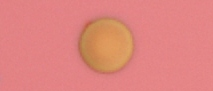
\includegraphics[scale=1.2,trim=1.25cm .45cm 1.25cm .45cm,clip]{Figs_Friction/SB03-2.jpg}};
	\end{scope}
	
	%The SiO2
	\filldraw[sio2] (-\edge,0) -- (-\radius, 0) -- (-\radius, -\topthick) -- (-\edge, -\topthick);
	\filldraw[sio2] (\edge,0) -- (\radius, 0) -- (\radius, -\topthick) -- (\edge, -\topthick);
	
	%The Si
	\fill[fill=black!20!white]
		(-\edge,-\topthick) -- (-\radius,-\topthick) 
		\foreach \i in {0,...,15}
			{-- (-\radius, -\topthick-\i*\srad) .. controls (-\radius-\srad/4, -\topthick-\srad/4-\i*\srad) and (-\radius-\srad/4, -\topthick-3*\srad/4-\i*\srad) ..
			(-\radius,-\topthick-\srad-\i*\srad) }
		-- (-\radius, -\topthick-\botthick) node[anchor=south west] {$P_0$} -- 
		(\radius, -\topthick-\botthick) 
		\foreach \j in {15,14,...,0}
			{-- (\radius, -\topthick-\srad-\j*\srad) .. controls (\radius+\srad/4, -\topthick-3*\srad/4-\j*\srad) and (\radius+\srad/4, -\topthick-\srad/4-\j*\srad) ..
			(\radius,-\topthick-\j*\srad) }
		 -- (\edge, -\topthick) -- 
		(\edge, -\topthick-\botthick-\basethick) -- (-\edge, -\topthick-\botthick-\basethick) [draw=none]-- cycle ;
	
	\draw[siedge](-\edge,-\topthick) --(-\radius,-\topthick);
	\foreach \i in {1,...,16}
		\draw[yshift=-1*(\i-1)*\srad,siedge] (-\radius, -\topthick) .. controls (-\radius-\srad/4, -\topthick-\srad/4) and (-\radius-\srad/4, -\topthick-3*\srad/4) ..
			(-\radius,-\topthick-\srad);
	\draw[siedge] (-\radius, -\topthick-\botthick) -- (\radius, -\topthick-\botthick);
	\draw[siedge] (\radius, -\topthick) -- (\edge, -\topthick);
	\foreach \i in {1,...,16}
		\draw[yshift=-1*(\i-1)*\srad,siedge] (\radius, -\topthick) .. controls (\radius+\srad/4, -\topthick-\srad/4) and (\radius+\srad/4, -\topthick-3*\srad/4) ..
			(\radius,-\topthick-\srad);
	
	\node at (9,1.5) {$N_2$};
	
	%The Graphene on the top
	\draw[thick] (-\edge,\grup) -- (-\radius,\grup) node[anchor=south west]{$P>P_0$}  parabola bend (0,-.7 cm)  (\radius,\grup) -- (\edge,\grup);
	
	%Scale bar
	\draw[draw=black,ultra thick, xshift=\radius/2+\edge/2-2.5cm, yshift=-\botthick-\topthick-\basethick/2] (0,0) -- node[anchor=south] {$5 \ \mu m$}(5 cm, 0);
	
	%Dashed lines
	\draw[color=black!40!white,dashed] (-\edge,\grup+.5cm) -- (-\edge,\grup+4.5 cm);
	\draw[color=black!40!white,dashed] (\edge,\grup+.5cm) -- (\edge,\grup+4.5 cm);
\end{tikzpicture}
	\end{center}
	\caption[Schematic of devices used to measure graphene's sliding]{\label{fig:fri:device} Top: An optical image of a trilayer graphene-sealed microchamber. Bottom: Device cross-section schematic showing the microchamber etched 8 $\mathrm{\mu}$m into the underlying Si substrate and the supported graphene atop the 300 nm of thermal oxide.  Pictured to scale is the largest pressure induced deflection of the graphene achieved in any of the analyzed experiments.}
\end{figure}

\section{Raman G band strain response\label{sec:fri:Raman}}
Micro-Raman spectroscopy is a powerful tool to measure strain distributions in graph\-ene.
The Raman G band measures the zone center, in-plane optical phonons that are degenerate at zero strain \cite{Tuinstra1970,Ferrari2006}.
In the absence of shear strain, the G band shifts according to \cite{Huang2009}
\begin{equation}
	\Delta \omega_G=-\omega_0 \gamma(\epsilon_{r}+\epsilon_{t}) \pm \frac{1}{2} \beta (\epsilon_{r}-\epsilon_{t}) \ ,
\end{equation}
where $\epsilon_{r}$ and $\epsilon_{t}$ are the strain in the radial and tangential directions,  $\gamma$ is the Gr\"{u}neisen parameter and $\beta$ is the shear deformation potential which details the amount of splitting between the $G^+$ and $G^-$ bands.

Light scattered by the $G^+$ and $G^-$  bands has orthogonal linear polarizations \cite{Huang2009}.
To isolate the individual peaks spectra are often measured using linearly polarized light.
Here, however, spectra are measured with circularly polarized light unless otherwise noted.
This allows more data to be acquired because the $G^+$ and $G^-$ bands are measured simultaneously.
Figure \ref{fig:fri:circlelinear} shows experimental verification that the spectra taken using circular polarized light matches the sum of the $G^+$ and $G^-$ bands.
The $G^+$ and $G^-$ bands were measured in the usual way by setting the incident excitation along the radial strain direction and measuring the emitted spectra as a function of emission polarization.
By summing over the spectra taken with emitted polarization varied from -90 to 90 degrees in 20 degree steps, a spectra with equal contributions from $G^+$ and $G^-$ is created.
As shown in Figure \ref{fig:fri:circlelinear}, these derived spectra match the single spectra taken with circularly polarized light. 
This verifies that spectra measured with circularly polarized represent both the $G^+$ and $G^-$ bands.

\begin{figure}
	\begin{center}
	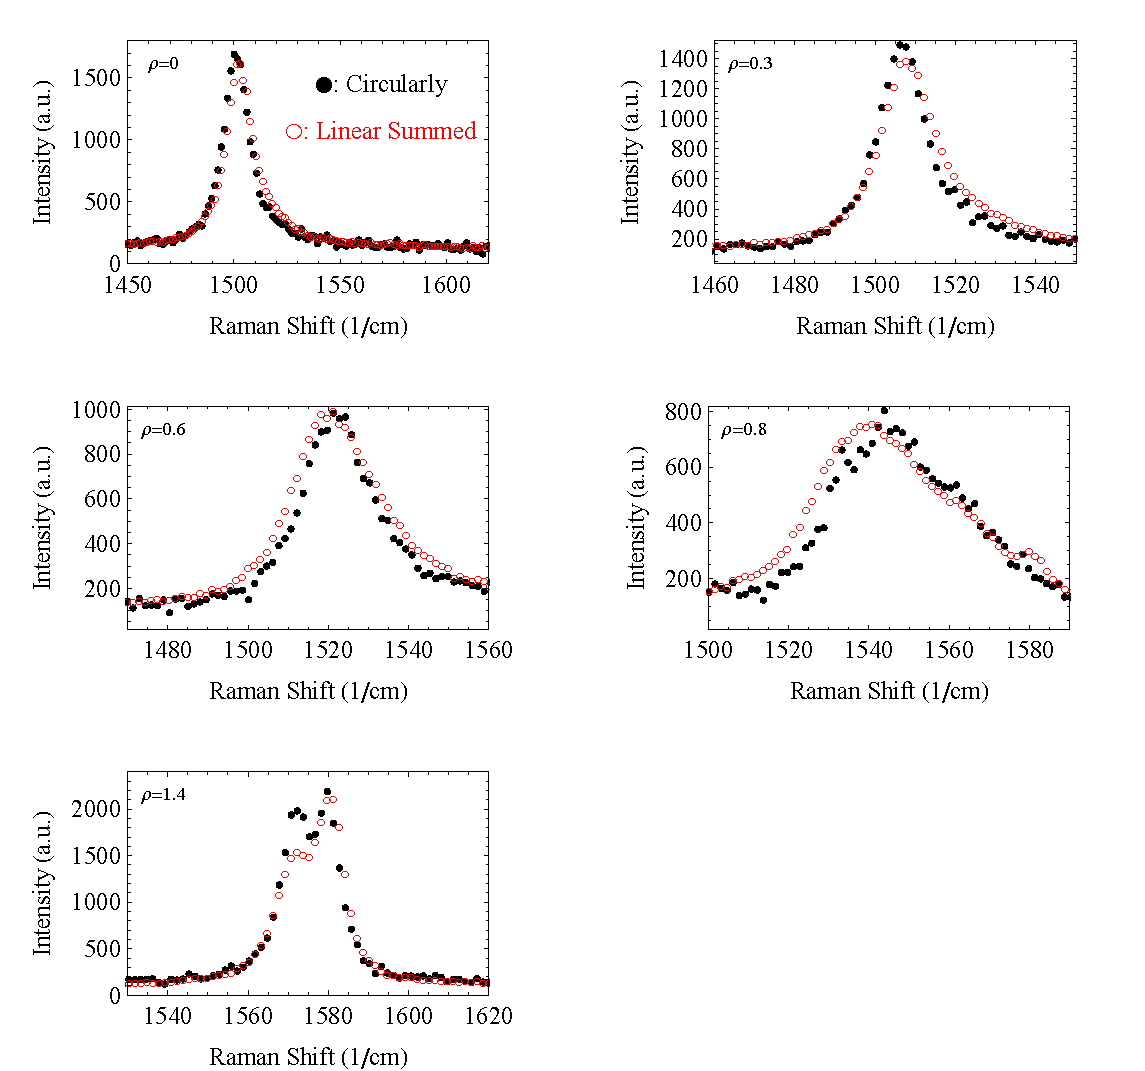
\includegraphics[scale=.75]{Figs_Friction/LinearvsCircular.pdf}
	\end{center}
	\caption[A comparison of Raman spectra measured using circularly and linearly polarized light]{\label{fig:fri:circlelinear}Comparison of Raman spectra measured using circularly and linearly polarized light. Measurements were taken at the labeled values of $\rho=r/R$ on a R=5 $\mathrm{\mu}$m graphene sealed microchamber under 0.80 MPa of applied absolute pressure. The black dots are spectrum measured using circularly polarized light. The red dots are the sum of spectra taken with outgoing polarizations varied between -90 to 90 degrees in 20 degree steps while the excitation is held in the $\hat x$ direction. Spectra are scaled to match intensities.}
\end{figure}

The local Raman response is measured inside an optically accessible pressure chamber with a focused laser beam while variable pressures up to 0.80 MPa are used to push the FLG into the microchamber.
Raman spectra are excited using the 514 nm line of an argon ion laser and collected using a Renishaw spectrometer with an 1800 lines/mm grating and a 63X, .7 NA, cover slip corrected objective.
The laser power in the pressure chamber was kept below 0.5 mW to avoid sample heating.
Optical access into the pressure chamber is through a 1 mm BK7 window.
The beam waist of the focused laser was measured to be $0.81 \pm .01 \ \mathrm{\mu m}$ by scanning a gold pad under the laser as shown in Figure \ref{fig:fri:waist}.

\begin{figure}
	\begin{center}
	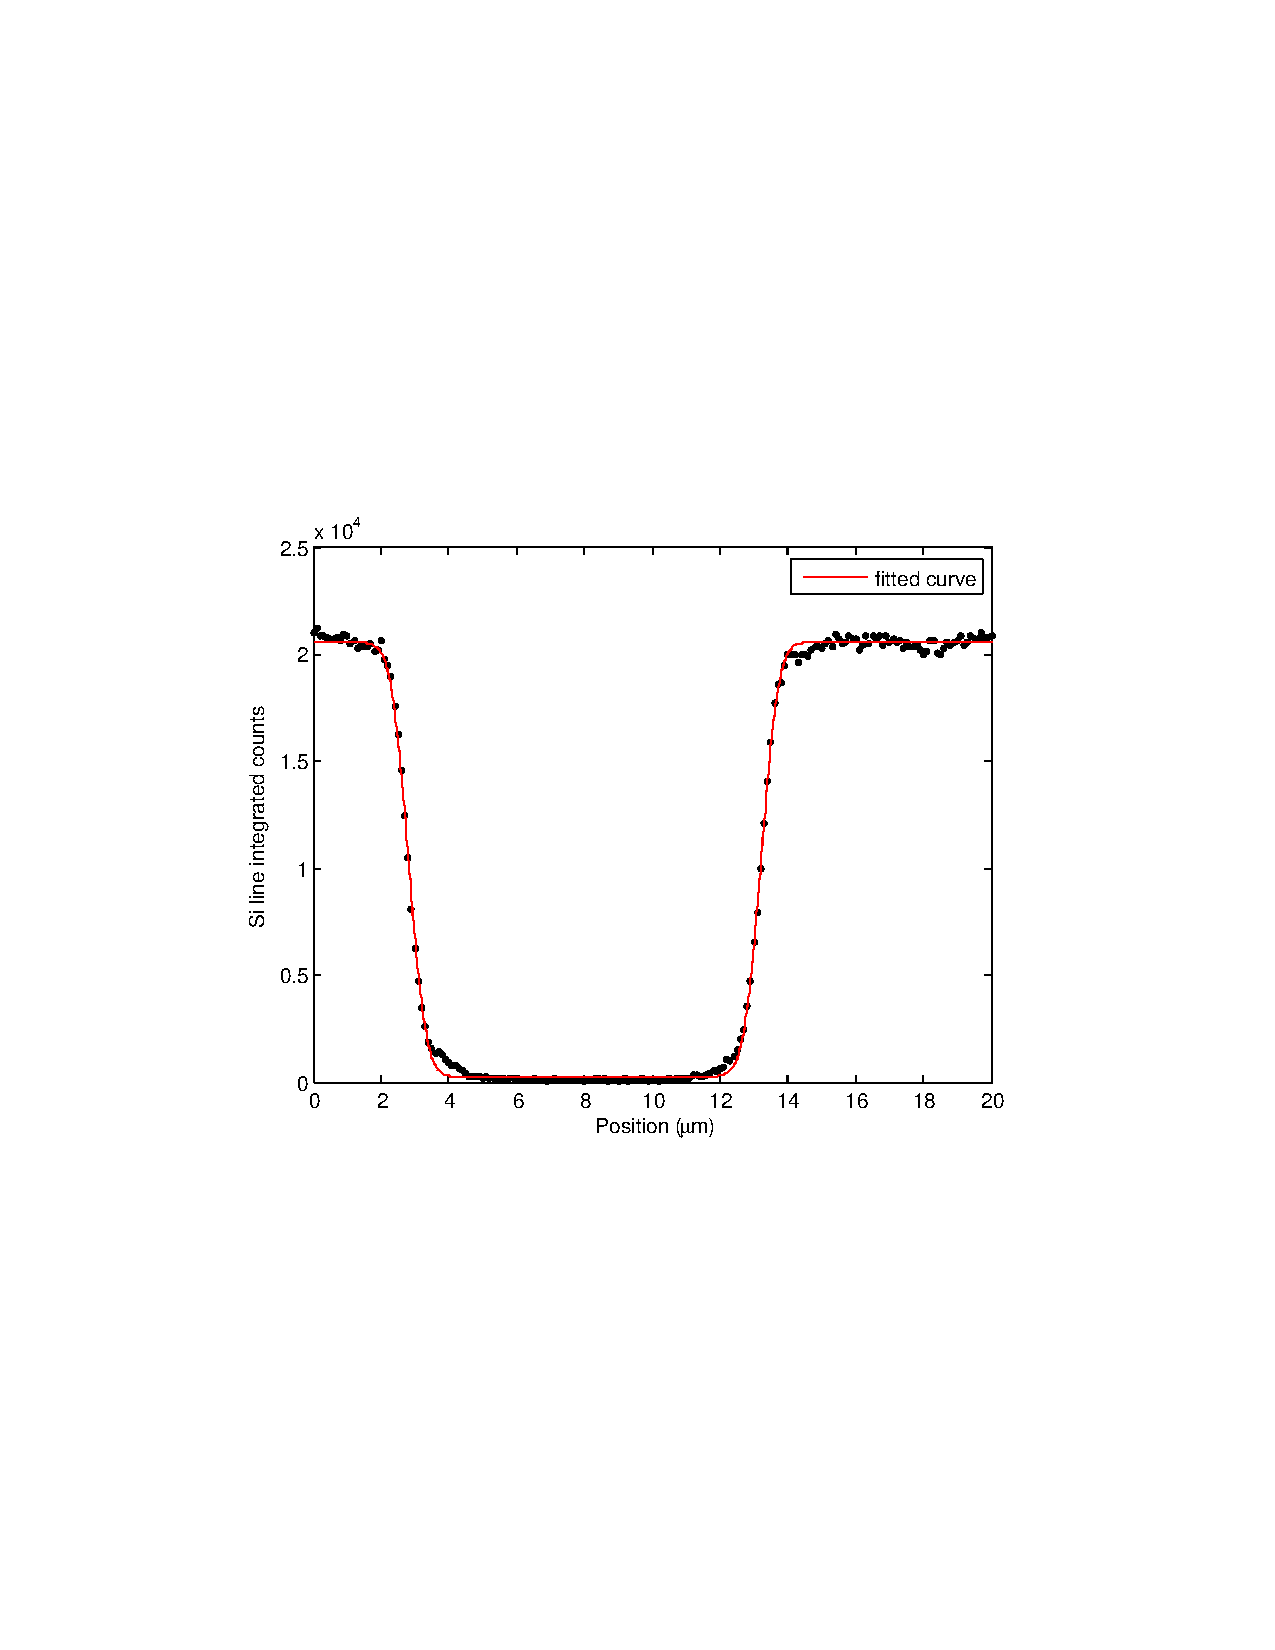
\includegraphics[scale=1]{Figs_Friction/SpotSize.pdf}
	\end{center}
	\caption[Determination of the beam waist of the focused laser in the pressure chamber]{\label{fig:fri:waist}Determination of the beam waist of the focused laser in the pressure chamber by scanning a sample with a gold pad under the focused beam while measuring the Si Raman line intensity. As the sharp edge of the gold pad moves under the laser, the Si line is blocked giving a measure of the beam size. Fitting the signal to an error function gives a beam waist of $0.81 \pm .01 \ \mu m$.}
\end{figure}

\section{Experimental Design}
A cross-section of one of the microchambers sealed with mechanically exfoliated FLG is depicted in Figure \ref{fig:fri:device}.
Microchambers are fabricated using standard optical lithographic methods to define holes ranging from 1 to 5 $\mathrm{\mu}$m in radii,  reactive ion etching to etch through the 300 nm thermal oxide layer, and deep reactive ion etching to etch roughly $8 \ \mathrm{\mu m}$ into the underlying silicon layer.
Before the graphene is mechanically exfoliated to seal the microchambers, the substrate is oxygen plasma ashed for 10 minutes at 300 sccm and 500 Watts to ensure the substrate is cleaned of any residues.
The number of graphene layers sealing each device was determined using Raman spectroscopy \cite{Ferrari2006} and optical contrast \cite{Blake2007,Casiraghi2007a}.

The large microchamber depth of $\sim 8 \ \mathrm{\mu m}$ is 10 times the largest FLG deflection of 700 nm.
This allows for the changes in internal pressure as the microchamber shrinks with pressure to be ignored.
It also enables longer measurement times because of slower leak-out rates through the silicon substrate.
To eliminate surface residues, the substrate was oxygen plasma ashed before FLG exfoliation.
It is important to note that different surface treatments may yield different sliding frictions providing a new degree of freedom in device engineering. 

Two complementary Raman measurements are performed \emph{in situ} to fully characterize the strain distributions.
First, as the absolute applied pressure is varied between atmospheric pressure (0.10 MPa) and 0.80 MPa, Raman spectra at the center of the microchamber are recorded.
Also, at selected pressures, Raman G band line scans with $ 0.5 \ \mathrm{\mu m}$ point spacing are taken across the microchamber.
The former is used to determine the pressure trapped inside the microchamber while the latter is used to determine the spatial distribution of the strain.
In conjunction with low force ($\approx 1 \ nN$) contact mode atomic force microscopy (AFM), the Raman spectra taken at the center of the microchamber reveal interesting ambient pressure behavior exhibited by the graphene sealed microchambers.

\subsection{Pressure trapped in microchambers\label{sec:fri:ambient}}
The ambient pressure behavior of the measured devices is split roughly evenly between two representative cases.
For half of the devices the pressure inside of the microchamber was greater than one atmosphere, as shown in the left side (a) of Figure \ref{fig:fri:ambient}.
Here, both the AFM and Raman measurements indicate that the pressure inside of the microchamber is greater than ambient.
The topographic image shows the graphene bulging out and the Raman G band response demonstrates that a non-zero gauge pressure is necessary for the G band to reach its greatest, or least strained, value.
By fitting the Raman data with the $p^{2/3}$ form predicted by the standard Hencky model for the strain at the center of the hole (blue dashed line), the internal pressure and unstrained G band position are found.

\begin{figure}
	\begin{center}
	\newcommand{\xs}{4.5 cm}
\newcommand{\totscale}{.6}
\newcommand{\afmscale}{.42}
\begin{tikzpicture}[scale=\totscale]
	%SB02-3
	\begin{scope}[xshift=\xs]
		\node at (0,0) {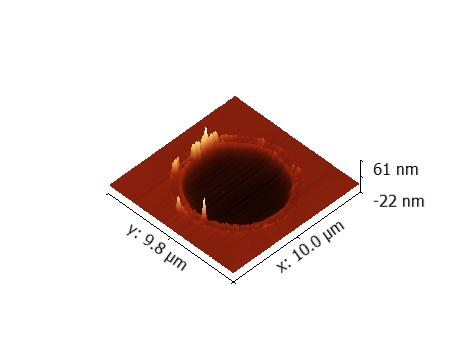
\includegraphics[scale=\afmscale]{Figs_Friction/AFM_SB02-3.jpg}};
		\node at (0,-4.5 cm) {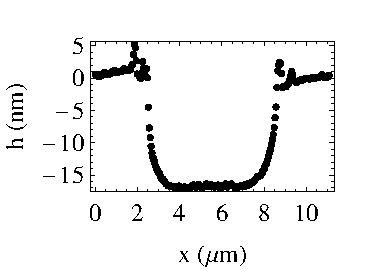
\includegraphics[scale=\totscale]{Figs_Friction/Section_SB02-3.pdf}};
		\node at (0,-10 cm) {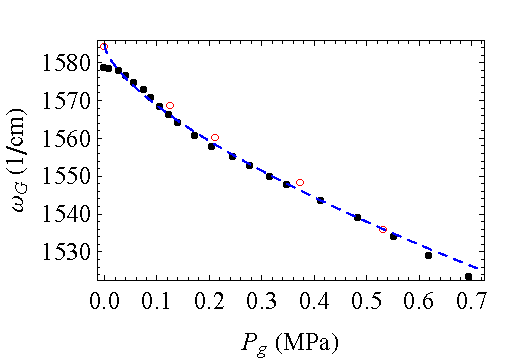
\includegraphics[scale=\totscale]{Figs_Friction/CenterFit_SB02-3.pdf}};
	\end{scope}
	%SB03-2b
	\begin{scope}[xshift=-\xs]
		\node at (0,0) {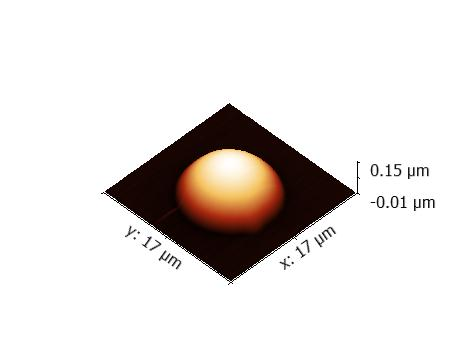
\includegraphics[scale=\afmscale]{Figs_Friction/AFM_SB03-2A.jpg}};
		\node at (0,-4.5 cm) {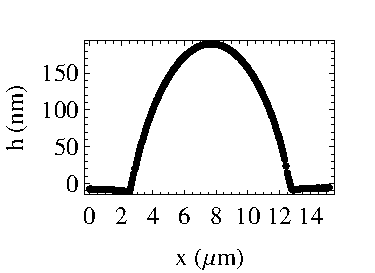
\includegraphics[scale=\totscale]{Figs_Friction/Section_SB03-2A.pdf}};
		\node at (0,-10 cm) {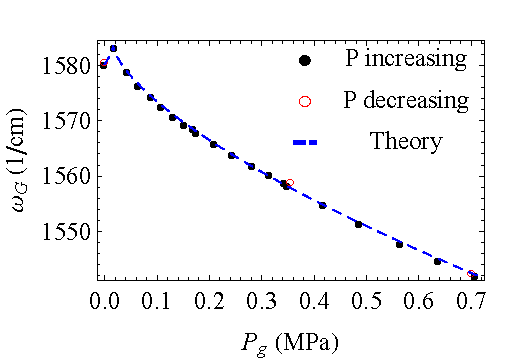
\includegraphics[scale=\totscale]{Figs_Friction/CenterFit_SB03-2A.pdf}};
	\end{scope}
	
	\node at (.7,1.75) [anchor=south west]{\textbf{b}  Snapped to side wall};
	\node at (-8,1.75) [anchor=south west]{\textbf{a} $P_0>P_a$};
\end{tikzpicture}
	\end{center}
	\caption[Characteristic ambient pressure behavior of FLG sealed microchambers]{\label{fig:fri:ambient}Characteristic ambient pressure behavior of FLG sealed microchambers. (Top) Low contact force ($\approx 1\ \mathrm{nN}$) AFM taken at ambient pressure with line cuts above (bottom) the center frequency of single Lorentzian fit spectra taken at the center of the hole as a function of the applied gauge pressure for (a) (left hand side) a 5 $\mathrm{\mu}$m radius trilayer sealed microchamber and (b) (right hand side) a 3 $\mathrm{\mu}$m radius monolayer sealed microchamber.}
\end{figure}

In the second half of the devices, the pressure inside the microchamber was an atmosphere, as shown on the right side (b) of Figure \ref{fig:fri:ambient}.
The AFM topography shows that the graphene is flat across the aperture indicating the internal pressure matches the ambient pressure.
The topography also shows that graphene is stuck to the walls of the microchamber for an AFM determined distance of roughly 7 nm.
Additionally, the Raman G band response in these devices shows interesting small strain behavior with increasing pressure which seems to be a result of graphene peeling off the side walls as it is pressurized.
At atmospheric pressure the G band is already red shifted due to pre-strain.
Increasing the gauge pressure to $\sim 0.1$ MPa causes a slower than expected downshift in the G band position.
However, when the gauge pressure is increased beyond $0.1$ MPa, the shift rate converges to the expected trend, $P^{2/3}$, and remains on this trend when the pressure is reduced back to atmospheric pressure.
This is consistent with the FLG unsticking from the walls as pressure is applied and remaining unstuck when the pressure returns to ambient pressure.
Values for friction are extracted from data taken at 0.17 MPa and above, well beyond the pressure domain where side wall sticking effects are observed.
For devices that behave in this way, the internal pressure is taken to be an atmosphere and the unstrained G band position is set as the G band position upon completing the pressure cycle.

Other groups have observed similar snap-to-sidewall behavior \cite{Lee2008,Bunch2008}.
Bunch and Dunn noted that the AFM measured distance over which FLG snaps to sidewalls may be overestimated \cite{Bunch2012}.
This position is supported by the comparison of the strain measured with Raman and the strain estimated from topography.
For a 3 $\mathrm{\mu}$m hole, a change in radius of 7 nm should generate .2\% strain whereas a Raman shift of -5 1/cm indicates a strain of .08\%.
Additionally, side wall sticking may explain the small Young's Modulus measured by Lee \textit{et al.} using a similar measurement over the a 0.1 MPa pressure range \cite{Lee2012}.

\section{Qualitative results}
Raman line scans over pressurized microchambers show that the supported graphene around the microchamber has slid inward toward the center.
Figure \ref{fig:fri:qualresults} shows the center frequency of single Lorentzian fits to the G band as a function of position across a 6 $\mathrm{\mu}$m diameter monolayer covered graphene sealed microchamber with applied absolute pressures of 0.45 and 0.80 MPa during three separate pressure cycles from atmospheric to 0.80 MPa.
As expected, as the suspended graphene is pushed down into the microchamber, the G band red shifts or softens from its unstrained value.
Unexpectedly, the G band of the supported graphene \emph{outside} the edge of the microchamber also shows softening, and thus significant strain.
The observed softening decreases with the distance from the edge of the microchamber until the G band returns to its unstrained energy.
This strain is real; the G band red shift cannot be attributed to the averaging over the finite spot size of the beam because the measured downshifts persist much further from the edge of the microchamber than the 0.83 $\mathrm{\mu}$m beam waist.
As the applied pressure increases, more strain is distributed outside of the microchamber causing both a larger redshift and a larger region over which the strain is distributed.
The strain distributed outside of the microchamber's edge is a clear indicator that the graphene is not rigidly fixed to the substrate outside of the microchamber.
Instead of a line force acting at the circumference of the microchamber to fix the graphene at the edge, there must be a distributed sliding frictional force, $f$, acting between the graphene and the substrate.

This behavior is reproducible, stable, and azimuthally symmetric.
The four 0.45 MPa line scans in Figure \ref{fig:fri:qualresults} include one line scan in the x direction for each of the first two pressure cycles and a line scan from both the x and y direction during the third pressure cycle.
The five 0.80 MPa line scans include one line scan in the x direction from the first pressure cycle, two sequential line scans in the x direction which took 35 minutes each from the second pressure cycle, and a line scan from both the x and y direction during the third pressure cycle.
Other than the development of a dimple at the center of the microchamber, the spectra and G band shifts are nearly identical.
This dimple is the result of laser deposition of dirt at the center of microchamber due to tens of hours of high pressure resolution, single point measurements.
An SEM image of the schmutz dimple is shown in the inset.
This dirt seems to stabilize the graphene underneath, reducing the strain in its vicinity.
Similar behavior is observed in each of the eight measured microchambers which have radii between 1.2 and 5 $\mu m$ and are covered with from one to three layers.

\begin{figure}
	\begin{center}
	\begin{tikzpicture}[scale=1]
	%The spectra
	\node at (0,0) {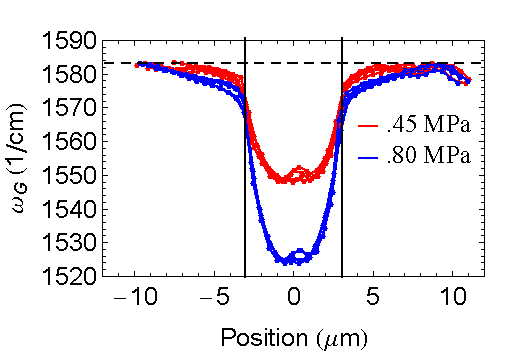
\includegraphics{Figs_Friction/QualLine.pdf}};
	
	%The picture of the hole
	\newcommand{\arrowlength}{1.5*.16*3.33 cm}
	\begin{scope}[xshift=-1.5 cm,yshift=0 cm]
		\node at (0,0) {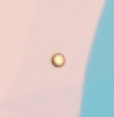
\includegraphics[scale=.75,angle=0,trim=9.75mm 8.5mm 8.5mm 10.25mm,clip]{Figs_Friction/SB02-3_cropped.jpg}};
		\draw[black,thick] (0,\arrowlength) -- (0,-\arrowlength) ;
		\draw[black,thick] (\arrowlength,0) -- (-\arrowlength,0);
	\end{scope}
	
	%The picture of the SEM dot
	\begin{scope}[xshift=2.6 cm,yshift=-.8 cm]
		\node at (0,0) {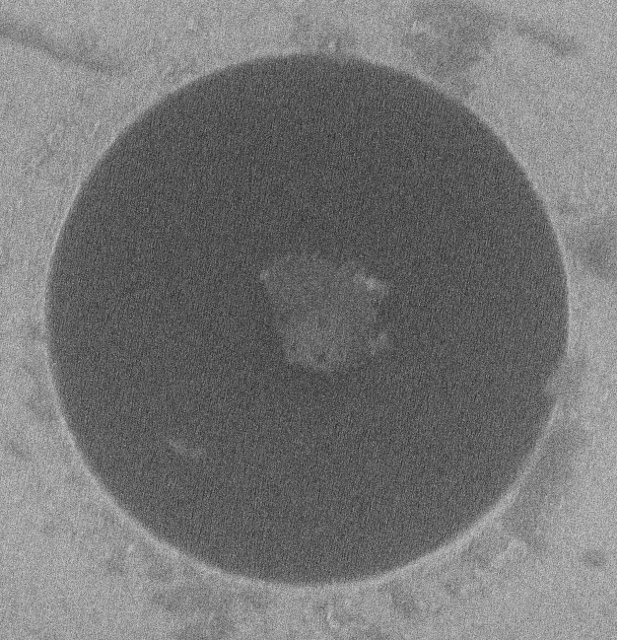
\includegraphics[width=.07 \textwidth]{Figs_Friction/SB02-3_05_SEM.jpg}};
	\end{scope}

\end{tikzpicture}
	\end{center}
	\caption[Qualitative observations of graphene sliding]{\label{fig:fri:qualresults} Qualitative observations of graphene sliding.  The frequency shift of the Raman G band as a function of position for four line scans taken at 0.45 MPa and five line scans taken at 0.80 MPa from 3 separate pressure cycles scanned across a single 6 $\mathrm{\mu}$m diameter monolayer sealed microchamber. Each point represents the position of the center of a single Lorentzian fit to the Raman spectra at that position.  Solid vertical black lines are positioned at the edges of the microchamber and the dashed horizontal line indicates the zero strain position of the G band.  Data points are separated by $0.5 \ \mu m$; the focused beam has a waste of 0.81 $\mathrm{\mu}$m. Inset left is an optical image of the microchamber with line scan direction indicated. The bottom right inset is an SEM image of the device taken after all of the data was acquired.}
\end{figure}

To determine the nature of the strain outside of the microchamber, Raman spectra 2 $\mathrm{\mu}$m outside the edge of a 5 $\mathrm{\mu}$m radius monolayer covered microchamber were analyzed in detail using linearly polarized light.
As shown in Figure \ref{fig:fri:qualout}, there are two discrete peaks in the spectra at 1570.9 1/cm and 1581.3 1/cm which are tuned on and off by rotating the analyzer on the outgoing light.
The polarization dependence of the integrated peak areas is consistent with the orthogonality of the $G^+$ and $G^-$ peaks \cite{Huang2009}.
The peak positions indicate a tensile radial strain of 0.6\% and a compressive tangential strain of -0.3\% at this location.
The compressive tangential strain is expected: When an annulus of the supported FLG is pulled inward, its circumference shrinks and, if the adhesion energy between FLG and its substrate is large enough to suppress out-of-plane wrinkling, this shrinkage causes compressive tangential strain.

\begin{figure}
	\begin{center}
	\newcommand{\sscale}{.6}
\newcommand{\sscaler}{.3}
\begin{tikzpicture}[scale=\sscale]	
	%The picture of the hole with the desciption of phiin and phoout
	\newcommand{\arrowlength}{1 cm}
	\begin{scope}[xshift=-4 cm,yshift=0 cm]
		%The spectra
		\node at (0,0) {\includegraphics[scale=\sscale]{Figs_Friction/PolarForSi.pdf}};
		%The hole
		\newcommand{\hcent}{1 cm}
		\begin{scope}[xshift=-.9 cm,yshift=10.15 cm,>=stealth]
			\node at (0,0) {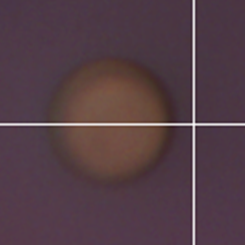
\includegraphics[scale=\sscaler ]{Figs_Friction/PolarPicture.png}};
			\draw[red,ultra thick,->] (\hcent-\arrowlength/2,-.03 cm) -- +(\arrowlength,0)  node[anchor=south west,fill=white]{$\phi_{in}$};
			\draw[green,ultra thick,->] (\hcent,-.03 cm) +(45:-\arrowlength/2) -- +(45:\arrowlength/2) node[anchor=south east, fill=white]{$\phi_{out}$};
		\end{scope}
	\end{scope}
	
	%The figure of the oscillating areas
	\begin{scope}[xshift=4 cm,yshift=0 cm]
		\node at (0,0) {\includegraphics[scale=\sscale]{Figs_Friction/ForSi_Areas.pdf}};
	\end{scope}
	
	\node at (.7,3) {\textbf{b}};
	\node at (-7,12.5) {\textbf{a}};
\end{tikzpicture}
	\end{center}
	\caption[Linearly polarized Raman spectra of supported graphene]{\label{fig:fri:qualout} (a) Linearly polarized Raman spectra of supported graphene taken 2 $\mathrm{\mu}$m outside a 5 $\mathrm{\mu}$m radius graphene sealed microchamber pressurized to 0.80 MPa absolute pressure with the incident light polarized in the $\hat x$ direction ($\phi=0$) and the outgoing light linearly analyzed at the labeled angle. (b) The areas under the 1570.9 1/cm and the 1581.3 1/cm peak as a function of outgoing analyzer angle in black and red, respectively fit with $\pi$ out-of-phase sine squared functions.}
\end{figure}

In the Raman and AFM experiments there is no evidence of the FLG wrinkling to relieve its compressive strain.
Shown in Figure \ref{fig:fri:cylindrical} is a partial Raman map of this 5 $\mathrm{\mu}$m radius monolayer covered microchamber at 0.80 MPa of applied pressure.
To generate the Raman maps Raman spectra were taken at each spatial location on the map.
Each spectra was fit with Lorentzians of energies $\omega^+$ and $\omega^-$ and the best fit energies were plotted as a function of the spatial location where the spectra was taken.
This two Lorentzian fit matches the characteristic two peak shape of the supported graphene shown in Figure \ref{fig:fri:circlelinear} for $\rho=1.4$.
Both maps in Figure \ref{fig:fri:cylindrical} were scaled to emphasize the shifts in the supported graphene peak positions.
As a result, the more highly strained suspended graphene appears black in the maps.
The $\omega^-$ Raman map, (a), shows very high radial symmetry while the $\omega^+$ map, (b), has slightly reduced symmetry.
At the highest point on the microchamber, there is a variation of around four wavenumbers in the $\omega^+$ map which could be due to small variations in local adhesion or could be due to nonuniform doping.
The degree of radial symmetry exhibited by both of these Raman maps is a strong indicator that the supported graphene is not wrinkling.
Since these Raman maps are for the microchamber with the largest diameter and thinnest thickness at the highest applied pressure, the compressive strains are the highest of any of the microchambers measured.
Thus, wrinkling in all other measured microchambers which have lower compressive strain can be precluded.

\begin{figure}
	\begin{center}
	\begin{tikzpicture}
	\node at (-4.75,2.75+5.5) {\textbf{(a)} $\omega^-$};
	\node at (0,5.5) {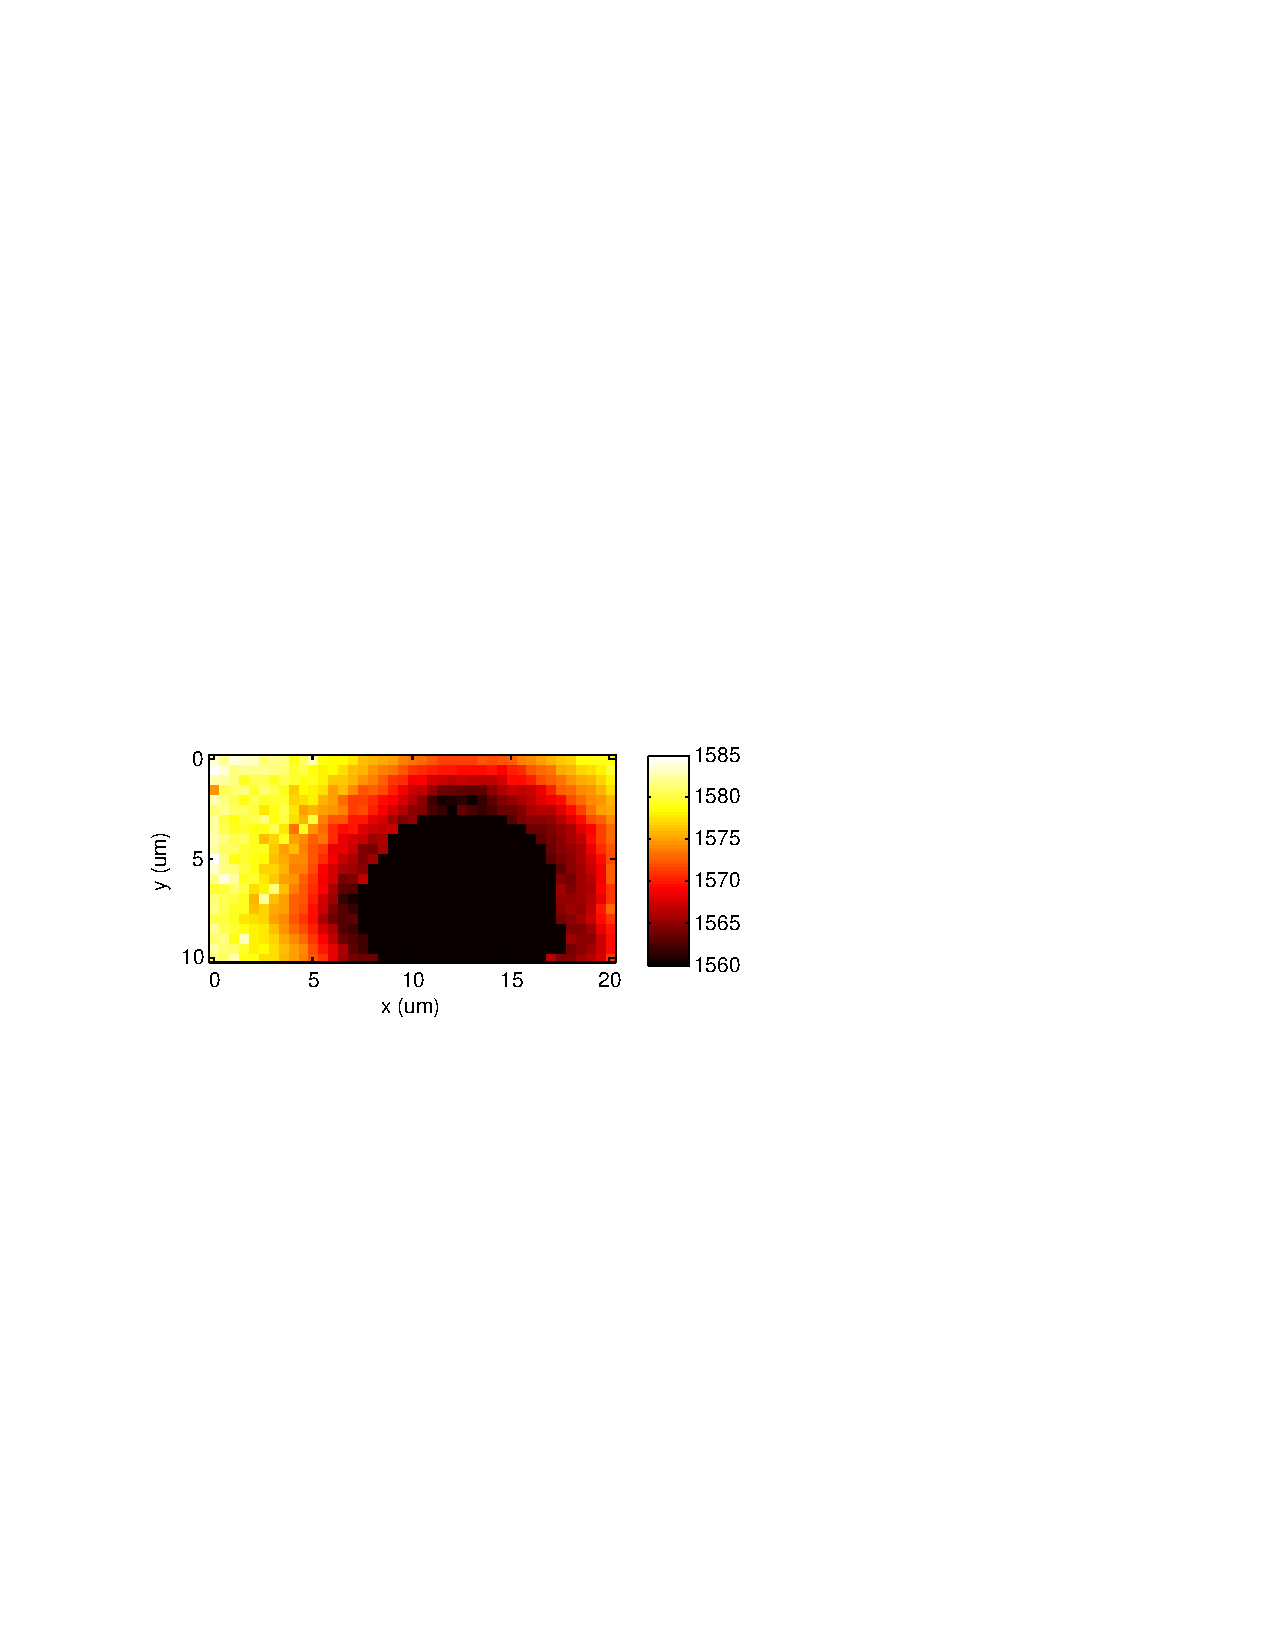
\includegraphics[scale=1]{Figs_Friction/x2.pdf}};
	\node at (-4.75,2.75) {\textbf{(b)} $\omega^+$};
	\node at (-.065,-.08) {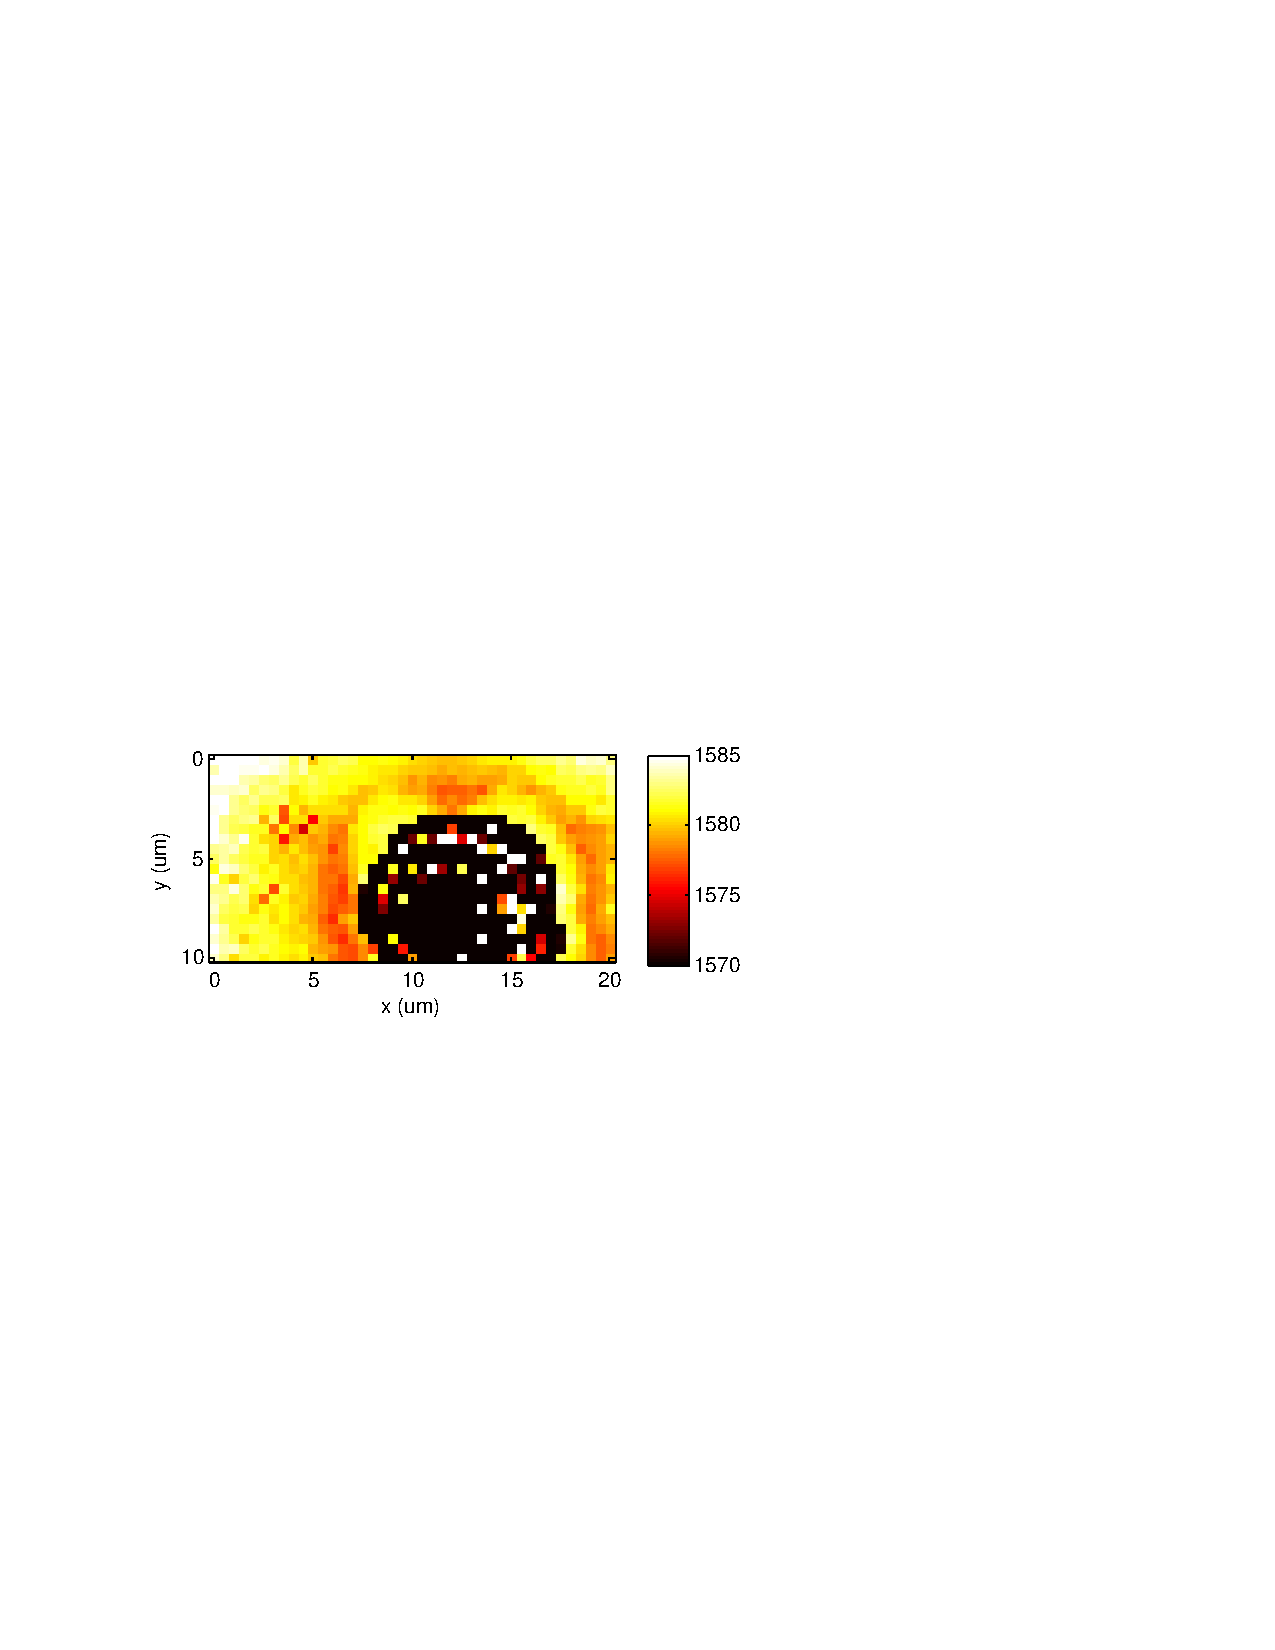
\includegraphics[scale=1]{Figs_Friction/x3.pdf}};
\end{tikzpicture}
	\end{center}
	\caption[Raman map of pressurized graphene sealed microchamber]{\label{fig:fri:cylindrical} Raman map of pressurized graphene sealed microchamber. (a) The $\omega^+$ peak and (b) $\omega^-$ peak for a 5 $\mathrm{\mu}$m radius graphene sealed microchamber pressurized to 0.80 MPa.  Color scale are set to emphasize the peak shifts experienced by the supported graphene.  The speckles in (b) appear because the suspended graphene spectra are not fit well by two Lorentzians.  Both maps show a high degree of radial symmetry inconsistent with the formation of wrinkles.}
\end{figure}

\section{Continuum model of strain distributions}
In this section, a continuum model to extract the sliding friction, $f$, from the Raman determined strain distributions is developed.
In 1915, Hencky proposed a continuum model for the non-linear pressure induced deflection of a thin circular plate with fixed boundary conditions \cite{Hencky1915,Fichter1997}.
This model has been successfully used to describe a variety of systems including inflatable membrane mirrors \cite{Meinel2000}, electrostatic actuators for micro gas pumps \cite{Zhang2011b}, and the topography of FLG bulging from sealed microchambers \cite{Koenig2011}.
However, the fixed boundary conditions assumed by this model preclude its application to the strain distributions observed here.
The fixed boundary conditions can be relaxed by matching the radial and tangential stresses inside the hole, derived from Hencky's model before the application of boundary conditions, to the radial and tangential stresses of the supported material outside of the hole found by including a sliding friction, $f$, acting against the radial displacement.
The stresses and, using Hooke's law, the strains, are then fully determined as a function of $\frac{\Delta P^2 E_{2D}}{f^3 R}$ where $R$ is the radius of the microchamber measured by AFM, $\Delta P$ is the differential pressure, and $E_{2D}$ is the 2D Young's modulus of FLG taken to be $n \times 340 \ N/m$ where n is the number of layers \cite{Lee2008,Koenig2011}.

Figure \ref{fig:fri:theory} compares the radial and tangential strains from the standard Hencky solution, the extended Hencky model derived here, and an atomistic, molecular dynamics model.
The solid lines of the extended model demonstrate the desired features; strain is distributed \emph{outside} of the hole with compressive tangential and tensile radial strain.
The strain distribution depends on the friction as expected: At constant pressure and radius, a greater sliding friction holds the graphene more firmly to the substrate surrounding the microchamber, and thereby increases $\epsilon_c$, the strain in the center of the microchamber, while also reducing $\rho_0$, the largest radial distance that the strain acts outside of the hole.
The extended model, with f=520 MPa, is in good agreement with the dots in Figure \ref{fig:fri:theory} that are the results of an atomistic molecular dynamics simulation of a 6 nm radius microchamber under 500 MPa of pressure performed using the open source simulation package LAMMPS \cite{plimptonLAMMPS,PlimptonJCP1995} developed at Sandia National Labs.

\begin{figure}
	\begin{center}
	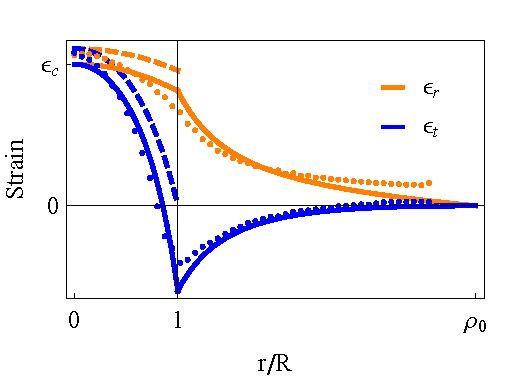
\includegraphics{Figs_Friction/Figure_3.pdf}
	\end{center}
	\caption[Theoretical strains in FLG sealed microchambers]{\label{fig:fri:theory} Theoretical strains in FLG sealed microchambers. Comparisons of the radial and tangential strains predicted by Hencky's model (dashed), the extended Hencky model that includes strain outside the microchamber for a sliding friction of f=520 MPa (solid), and atomistic simulations of a 6 nm radius microchamber with 500 MPa of applied pressure (dots). The extended Hencky model used to extract friction agrees very well with the atomistic model.}
\end{figure}

This work represents the first time that Hencky's model has been generalized to allow strain to be distributed outside of the microchamber's edge.
The derivations provides a framework for including the sliding of graphene over a rigid substrate in a continuum model.
This should be useful in applications such as the strain engineering of pseudo magnetic fields.
For those interested, a full derivation of the extended Hencky model as well as a detailed description of the atomistic modeling is included in the next sections.

\subsection{Detailed derivation of the extended Hencky model}
To derive the extended Hencky model the general forms of the stress inside and outside of the hole will be derived, and then the boundary condition will be determined and applied.
The resulting solution will be a function of the dimensionless loading parameter, $q=\frac{\Delta PR}{E_{2D}}$, and the dimensionless friction coefficient $F=Rf/E_{2D}$ in the combination $q^{2/3}/F$.
This means that large dimensionless loading, $q^{2/3}$, causes the same effects as  small friction, $F$;  pushing hard has the same effect as sliding easily.
A simple analytic relationship does not exist between  $q^{2/3}/F$ and the two parameters which define the shape of the strain profile: the distance over which the strain spreads outside of the hole, $\rho_0$, and the coefficient of stress at the center of the hole, $b_0$.
However, these can be easily solved for analytically.

Throughout this section graphene is treated in the continuum limit as a thin plate: A solid which is much thinner in one dimension than the other two.
Assuming that there is no shear, the stress-strain relationship for the thin plate is the same inside and outside the hole \cite{Landau1986} 
\begin{align}
	\epsilon_r&=\sigma_r-\nu \sigma_t \label{eq:fri:esr}\\
	\epsilon_t&=\sigma_t-\nu \sigma_r \label{eq:fri:est} \ ,
\end{align}
where $\nu$ is the Poisson Ratio and $\sigma_r$ and $\sigma_t$ are the dimensionless radial and tangential stresses given by the stress divided by the effective 3D Young's modulus ($E_{3D}=E_{2D}/t$ where $t$ is the thickness).

Both the strain-displacement and the governing equations, however, depend on the region of interest.
For the suspended material, the plate flexes down into the hole as pressure is applied.
The resulting strain-displacement relationships are
\begin{align}
	\epsilon_r^i&=\frac{dU}{d\rho}+\frac{1}{2} (\frac{dW}{d\rho})^2 \label{eq:fri:edri}\\
	\epsilon_t^i&=\frac{U}{\rho} \label{eq:fri:edti} \ ,
\end{align}
where $U$ is the dimensionless radial deflection, $W$ is the dimensionless out of plane deflection, and $\rho$ is the dimensionless radius, all of which are made dimensionless by dividing by the radius of the hole.
The governing equations inside the hole are calculated by balancing the forces on a radial element.
The stresses and pressure acting on such an element are shown in Figure \ref{fig:fri:stressfigurei}.
Using the area of the radial element ($r dr d\theta$) to convert the pressure to a force, and the cross sectional area to convert the strains into forces results in the two governing equations
\begin{align}
	\sigma_t^i&=\frac{d}{d \rho}(\rho \sigma_r^i) \label{eq:fri:g1i}\\
	\sigma_r^i \frac{dW}{d \rho}&=-\rho \frac{q}{2} \label{eq:fri:g2i} \ .
\end{align}
the first from radial equilibrium and the second from lateral equilibrium.
These six equations can be combined to form a single differential equation for $\sigma_r$
\begin{equation}
	\frac{1}{8} \rho q^2+ (\sigma_r^i)^2 \frac{d}{d\rho}[\sigma_r^i+\frac{d}{d\rho}(\rho \sigma_r^i)]=0 \ .
	\label{eq:fri:comboin}
\end{equation}
This is most easily found by using Equation \ref{eq:fri:g1i} and then Equation \ref{eq:fri:g2i} in the combination of Equations: $[(\ref{eq:fri:edri}) \rightarrow (\ref{eq:fri:esr})]-\frac{d}{d \rho}\rho[(\ref{eq:fri:edti})\rightarrow(\ref{eq:fri:est})]$.
Once this equation is used to solve for $\sigma_r$, Equations \ref{eq:fri:g1i}, \ref{eq:fri:esr}, and \ref{eq:fri:est} allow the easy determination of $\sigma_t$, $\epsilon_r$, and $\epsilon_t$.
Since there is no analytic solution to this differential equation, so, following Hencky's lead, a series expansion of the radial stress even in powers of $\rho$ to match symmetry is assumed
\begin{equation}
	\sigma_r^i=\frac{1}{4} q^{2/3} \sum_{n=0}^{\infty} b_{2n} \rho^{2n} \ .
\end{equation}
When used in eqn. \ref{eq:fri:comboin} all of the higher order coefficients are determined in terms of one free parameter, $b_0$, the stress coefficient at the center of the hole.
To this point the derivation has not deviated from Hencky's original work.
However, instead of continuing forward to determine the value of $b_0$ by requiring that there is no radial deflection at the edge of the hole, $b_0$ will be left as a free parameter to match to the strain outside of the hole, which is now derive.

\begin{figure}
	\begin{center}
	\newcommand{\halfangle}{10}
\begin{tikzpicture}[scale=2]
	%The radial equilibrium
	\begin{scope}[xshift=-4.5 cm]
		%The bisected dotted lines
		\begin{scope}[dashed,gray,very thin]
			\draw (0,0) -- (\halfangle:1.5 cm);
			\draw (0,0) -- (-\halfangle:1.5 cm);
		\end{scope}
		%Draw the area element
		\filldraw[fill=gray!10,draw=black] (-\halfangle:1.5 cm)  arc(-\halfangle:\halfangle:1.5 cm) -- (\halfangle:2 cm) arc(\halfangle:-\halfangle:2 cm) -- cycle;
		%Draw the force lines and labels
		\begin{scope}[->, blue!50!black,>=stealth]
			\draw (0:2 cm) -- +(0:.25 cm) node[anchor=west]{$N_r+\frac{dN_r}{dr} dr$};
			\draw (0:1.5 cm) -- +(0:-.25 cm) node[anchor=east]{$N_r$};
			\draw (\halfangle:1.75 cm) -- +(90+\halfangle:.25 cm) node[anchor=south east]{$N_t$};
			\draw (-\halfangle:1.75 cm) -- +(-90-\halfangle:.25 cm) node[anchor=north east]{$N_t$};
		\end{scope}
		\draw (.25,.75 cm) node{Top:};
	\end{scope}
	
	%The lateral equilibrium
	\begin{scope}[->, blue!50!black,>=stealth]
		\draw (0,0) -- (20:-.25 cm) node[anchor=north east]{$N_r$};
		\draw[black,thick,-] (20:0 cm) -- ++(20:.5 cm);
		\draw (20:.5 cm)  -- ++(20:.25 cm) node[anchor=west]{$N_r+\frac{dN_r}{dr} dr$};
		\draw (20:.25 cm) -- ++(90:.25 cm) node[anchor=west]{$P$};
		\filldraw (0,0) circle(.5pt);
		\filldraw (20:.5 cm) circle(.5pt);
		\filldraw (20:.25 cm) circle(.5pt);
	\end{scope}
	\draw (-.25,.75 cm) node{Side:};
	
\end{tikzpicture}
	\end{center}
	\caption[Force diagram of the suspended section of a pressurized graphene sealed microchamber]{\label{fig:fri:stressfigurei} Force diagram of the suspended section ($\rho<1$) of a pressurized graphene sealed microchamber. Depicted are the stresses, $N_r=E_{3D} \sigma_r$ and $N_t=E_{3D} \sigma_t$, and pressure, $P$, which act on a radial area element as viewed from the top and side.}
\end{figure}

Outside of the hole the plate is constrained to move in the x-y plane, radial symmetry is preserved, and friction is present. 
The stress strain relationships (eqns. \ref{eq:fri:esr} and \ref{eq:fri:est}) are for a thin plate with no shear, and thus, apply equally well outside the hole as inside.
The strain displacement relationships are based on the geometry of a general radially symmetric differential element.
The only change that needs to be made to these is the elimination of the out of plane motion, 
\begin{align}
	\epsilon_r^o&=\frac{dU}{d\rho} \label{eq:fri:edro}\\
	\epsilon_t^o&=\frac{U}{\rho} \label{eq:fri:edto} \ .
\end{align}
For sufficiently negative $\epsilon_t$, the plate is expected to buckle out-of-plane, forming wrinkles.
However, in the experimental regime there is no evidence for these effects.
The forces acting on the plate are different inside and outside the hole, and thus, so are the governing equations.
The stresses and forces acting on the graphene outside of the hole are shown in Figure \ref{fig:fri:stressfigureo}.
The interaction between the plate and its underlying substrate is included via the frictional force per unit area, $f$, which is pointed to oppose the radial stresses outside of the hole.
If there were a component of friction acting against the tangential strain, it would go as $d \theta^2$ rendering it negligible.
One power of $d \theta$ from the resultant and the other from the area element.
Care needs to be taken in this mathematical treatment because this friction term does not turn off when the stress goes to zero.
Instead, it works in positive feedback amplifying the stress. 
As a result, the stresses are only physical until they decay to zero at a position $\rho_0$.
The governing equation outside the hole is then
\begin{equation}
	\sigma_t^o=\frac{d}{d\rho}(\rho \sigma_r^o)+F \rho  \ .
	\label{eq:fri:g1o}
\end{equation}
Again these equations can be combined to form a single differential equation for $\sigma_r$.
The easiest way to do this is by using Equation \ref{eq:fri:g1o} twice in the combination of Equations: $[(\ref{eq:fri:edro}) \rightarrow (\ref{eq:fri:esr})]-\frac{d}{d \rho}\rho[(\ref{eq:fri:edto})\rightarrow(\ref{eq:fri:est})]$.
The result is
\begin{equation}
	\frac{d}{d\rho}[\sigma_r^o+\frac{d}{d\rho}(\rho \sigma_r^o)]=-(2+\nu) F \ .
	\label{eq:fri:comboout}
\end{equation}
Unlike the situation for $\rho<1$, this equation can be solved exactly.
The general result for the radial and tangential stresses are
\begin{align}
	\sigma_r^o&=(2+\nu)F(-\frac{\rho}{3}-\frac{c_2}{2 \rho^2})+c_1 \\
	\sigma_t^o&=(2+\nu)F(-\rho \frac{1+2 \nu}{3(2+\nu)}+\frac{c_2}{2 \rho^2})+c_1 \ ,
\end{align}
where the tangential stress was solved for using Equation \ref{eq:fri:g1o}.
To reduce the number of free coefficients, the radial and tangential strains are both forced to come to zero at the position $\rho_0$.
This natural restriction imposes a limit on the region where the theory gives physical results.
For $\rho>\rho_0$, the mathematical friction persists even though there is no stress, yielding unphysical results.
For these regions, the stresses are taken to be zero.
Applying this restriction gives $c_2=\rho_0^3 \frac{\nu-1}{3(2+\nu)}$ and $c_1=\rho_0 \frac{1+\nu}{2} F$.
This defines in closed form the strains for $\rho>1$ as a function of one free parameter, $\rho_0$.

\begin{figure}
	\begin{center}
	\newcommand{\halfangle}{10}
\begin{tikzpicture}[scale=2]
	%The bisected dotted lines
	\begin{scope}[dashed,gray,very thin]
		\draw (0,0) -- (\halfangle:1.5 cm);
		\draw (0,0) -- (-\halfangle:1.5 cm);
	\end{scope}
	%Draw the area element
	\filldraw[fill=gray!10,draw=black] (-\halfangle:1.5 cm)  arc(-\halfangle:\halfangle:1.5 cm) -- (\halfangle:2 cm) arc(\halfangle:-\halfangle:2 cm) -- cycle;
	%Draw the force lines and labels
	\begin{scope}[->, blue!50!black,>=stealth]
		\draw (0:2 cm) -- +(0:.25 cm) node[anchor=west]{$N_r+\frac{dN_r}{dr} dr$};
		\draw (0:1.5 cm) -- +(0:-.25 cm) node[anchor=east]{$N_r$};
		\draw (\halfangle:1.75 cm) -- +(90+\halfangle:.25 cm) node[anchor=south east]{$N_t$};
		\draw (-\halfangle:1.75 cm) -- +(-90-\halfangle:.25 cm) node[anchor=north east]{$N_t$};
		\filldraw[red!40!black] (1.75,0) circle(.5pt);
		\draw[red!40!black] (1.75,0) -- +(.15,0) node[anchor=south east]{$f$};
	\end{scope}
\end{tikzpicture}
	\end{center}
	\caption[Force diagram of the supported section of a pressurized graphene sealed microchamber]{\label{fig:fri:stressfigureo} Force diagram of the supported section ($\rho>1$) of a pressurized graphene sealed microchamber.  Depicted are the stresses, $N_r=E_{3D} \sigma_r$ and $N_t=E_{3D} \sigma_t$, and friction, $f$, which act on a radial area element.}
\end{figure}

Next, the boundary condition for the stresses at the edge of the hole will be determined so that the stresses can be matched across the boundary.
The stress is related to the force per unit area through a divergence operation
\begin{equation}
	F_i=\frac{\partial N_{ik}}{\partial x_k} \ ,
\end{equation}
where $F_i$ is the applied force per unit volume in the $i$ direction, $N_{ik}$ is the strain tensor, and repeated indices are summed over.
Integrating the equations and using the divergence theorem gives
\begin{equation}
	\int_V F_i \ dV=\oint_S \sigma_{ik} \ df_k \ .
\end{equation}
Hence, the total force acting on a volume entity is given by the surface integral of the stress.
A symmeterized volume element that spans the edge of the hole is shown in Figure \ref{fig:fri:egestress}.
In the limit that the width of the volume element, $\epsilon$, goes to zero the contributions from the surface forces, $f$ and $P$, also go to zero and so must the surface integral of the stresses.
This would not be the case if these were 1D edge forces.
The undrawn tangential stresses also go to zero since the cross section that they act on, $\epsilon t$ where $t$ is the thickness, goes to zero as well. 
Thus, the remaining stresses must be equal,
\begin{equation}
	N_r^i=N_r^o \ .
\end{equation}
The boundary condition on the tangential stress is found by the requirement that the radial displacement, $U$, must be continuous.
If it were not, the material on one side of the discontinuity would separate from the material on the other side leaving a gap.
If $U$ is continuous, so must $\epsilon_t$ be by eqns. \ref{eq:fri:edti} and \ref{eq:fri:edto}.
Finally, if $\epsilon_t$ and $N_r$ are continuous, so must $N_t$ be by equation \ref{eq:fri:est}.
This proves that the radial and tangential stresses must be continuous over the edge of the hole.

\begin{figure}
	\begin{center}
	\newcommand{\halfangle}{10}
\newcommand{\dr}{.3 cm}
\newcommand{\rbeg}{1.5 cm}
\newcommand{\Larrow}{.25 cm}
\begin{tikzpicture}[scale=2]
	%The bisected dotted lines
	\begin{scope}[dashed,gray,very thin]
		\draw (0,0) -- (\halfangle:\rbeg);
		\draw (0,0) -- (-\halfangle:\rbeg);
	\end{scope}
	%Draw the area element
	\filldraw[fill=gray!10,draw=black] (-\halfangle:\rbeg)  arc(-\halfangle:\halfangle:\rbeg) -- (\halfangle:\rbeg+\dr) arc(\halfangle:-\halfangle:\rbeg+\dr) -- cycle;
	%Draw the edge of the hole
	\draw[dotted,thick] (-4*\halfangle:\rbeg+\dr/2) arc(-4*\halfangle:4*\halfangle:\rbeg+\dr/2) node[anchor=south]{$\rho=1$};
	%Draw the force lines and labels
	\begin{scope}[->, blue!50!black,>=stealth]
		\draw (0:\rbeg+\dr) -- +(0:\Larrow) node[anchor=west]{$N_r^o$};
		\draw (0:\rbeg) -- +(0:-\Larrow) node[anchor=east]{$N_r^i$};
		\filldraw[red!40!black] (\rbeg+\dr*3/4,0) circle(.5pt);
		\draw[red!40!black] (\rbeg+\dr*3/4,0) -- +(.1,0) node[anchor=south east]{$f$};
		\filldraw[red!40!black] (\rbeg+\dr*1/4,0) circle(.5pt) node[anchor=north]{$P$};
	\end{scope}
	%Draw the width of the element
	\draw[<->,black,>=stealth] (\halfangle*5/4:\rbeg) -- node[anchor=south]{$\epsilon \rightarrow 0$} +(\halfangle*5/4:\dr);
\end{tikzpicture}
	\end{center}
	\caption[The boundary condition at the edge of the microchamber]{\label{fig:fri:egestress}The boundary condition at the edge of the microchamber is determined by the stresses and forces acting on a thin, symmetrized volume element which spans the edge of the hole.  The tangential strains inside and outside are ignored because their contribution goes to zero as the width of the element, $\epsilon$ goes to zero.  $P$ is the pressure which acts out of plane.}
\end{figure}

All of the necessary relationships have now been derived.
The series solution for the stresses for $\rho<1$ as a function of the dimensionless loading, $q$, are known with $b_0$, the stress at the center, a free parameter.
Similarly, the closed form solution for the stresses for $\rho>1$ as a function of the dimensionless friction, $F$, have been found, with $\rho_0$, the furthest distance the stress spreads, as a free parameter.
The derived boundary conditions at $\rho=1$ can now be applied 
\begin{align}
	\sigma_r^i(\rho=1)&=\sigma_r^o(\rho=1) \nonumber \\
	\sigma_t^i(\rho=1)&=\sigma_t^o(\rho=1) \ . \label{eq:fri:BCs}
\end{align}
This sets the value of $\rho_0$ and $b_0$ in terms of $q^{2/3}/F$.
Regrettably, the series form of the solution inside of the hole makes the presentation of an exact expression for $\rho_0$ and $b_0$ impossible.
Numerical solutions for the values of $\rho_0$ and $b_0$ are presented in Figures \ref{fig:fri:rho0b0} for graphite's Poisson ratio of 0.165 \cite{Blakslee1970}.
As the friction increases or the dimensionless loading coefficient decreases, $q^{2/3}/F$ decreases, and $\rho_0$ decreases toward unity, indicating that no strain distribution outside of the hole.
At the same time $b_0$ increases toward the limiting value of 1.66, the result for the original Hencky model which assumes perfectly fixed boundary conditions at the edge of the hole. 

\begin{figure}
	\begin{center}
	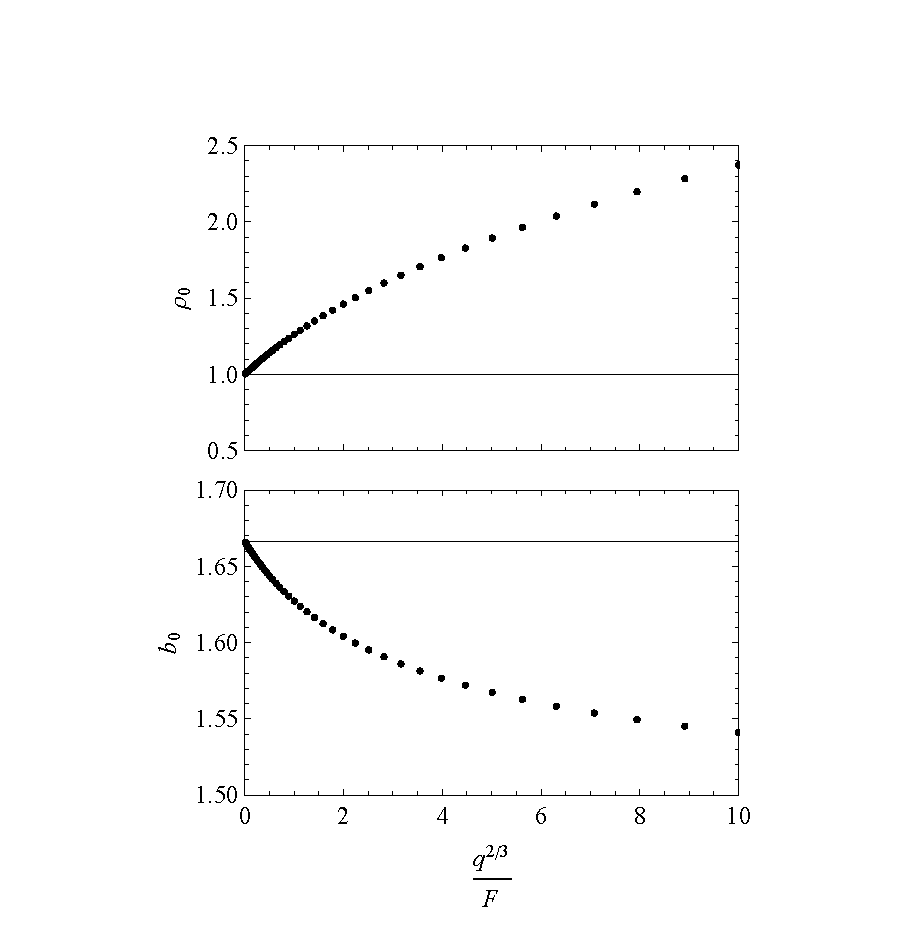
\includegraphics{Figs_Friction/b0rho0.pdf}
	\end{center}
	\caption[Numerical solutions for the values of $\rho_0$ and $b_0$]{\label{fig:fri:rho0b0} Numerical solutions for the values of $\rho_0$ and $b_0$, the furthest normalized radii that the strain reaches and the coefficient for the strain at the center of the hole, respectively. Note the large friction convergence to the values of the original Hencky model, $\rho_0 = 1$ and $b_0=1.66$.}
\end{figure}

This completes the derivation of the extended Hencky model.
The shape of the strain distributions shown in Figure \ref{fig:fri:theory} has been determined along with the pressure, friction, radius, and layer thickness dependencies shown in Figure \ref{fig:fri:rho0b0}.

\subsection{Detailed description of the Atomistic model}
In this section the atomistic model used to verify the extended Hencky continuum model is discussed.
Classical molecular dynamics simulations (MD) were performed using open source simulation package LAMMPS \cite{plimptonLAMMPS,PlimptonJCP1995} developed at Sandia National Labs.
The model used argon gas to compress a graphene monolayer that lies atop an amorphous silicon dioxide substrate, as illustrated in Figure \ref{fig:fri:MD}.
The substrate had dimensions 46 x 46 x 3 nm with a 6 nm radius hole in the center.
A circular graphene monolayer with radius 22 nm was placed on top of the hole in the substrate and argon atoms were randomly distributed within the simulation box after relaxation of the graphene-substrate system.
There were 562,110 atoms in total, with the simulation run in parallel for maximum computational efficiency.

The covalent carbon bonds were modeled using the AIREBO \cite{stuartJCP2000} potential, which has been shown to have good accuracy in describing hydrocarbon systems \cite{qiNANO2010,zhaoJAP2010}.
The Tersoff \cite{tersoffPRB1988} potential was utilized for the Si-Si, Si-O and O-O interactions, while a Lenard-Jones potential was used for all other interactions with a cutoff distance of 8 \AA \ and the corresponding interaction parameters chosen as follows: $\epsilon_{Ar-Ar}$=0.0104 eV, $\sigma_{Ar-Ar}$=3.405 \AA \cite{RytkonenJchemp1998}; $\epsilon_{Ar-C}$=0.0123 eV, $\sigma_{Ar-C}$=3.573 \AA \cite{RobertNano1996}; $\epsilon_{Ar-Si}$=0.0028 eV, $\sigma_{Ar-Si}$=3.778 \AA \cite{LiPRA2010}; $\epsilon_{Ar-O}$=0.0058 eV, $\sigma_{Ar-O}$=3.3075 \AA \cite{EverittJCP1999}; $\epsilon_{Si-C}$=0.008909 eV, $\sigma_{Si-C}$=3.326 \AA \cite{OngPRB2010}; $\epsilon_{O-C}$=0.003442 eV, $\sigma_{O-C}$=3.001 \AA \cite{OngPRB2010}.
The Ar-Si and Ar-O interaction parameters were obtained using the standard Lorentz-Berthelot mixing rule.

\begin{figure}
	\begin{center}
	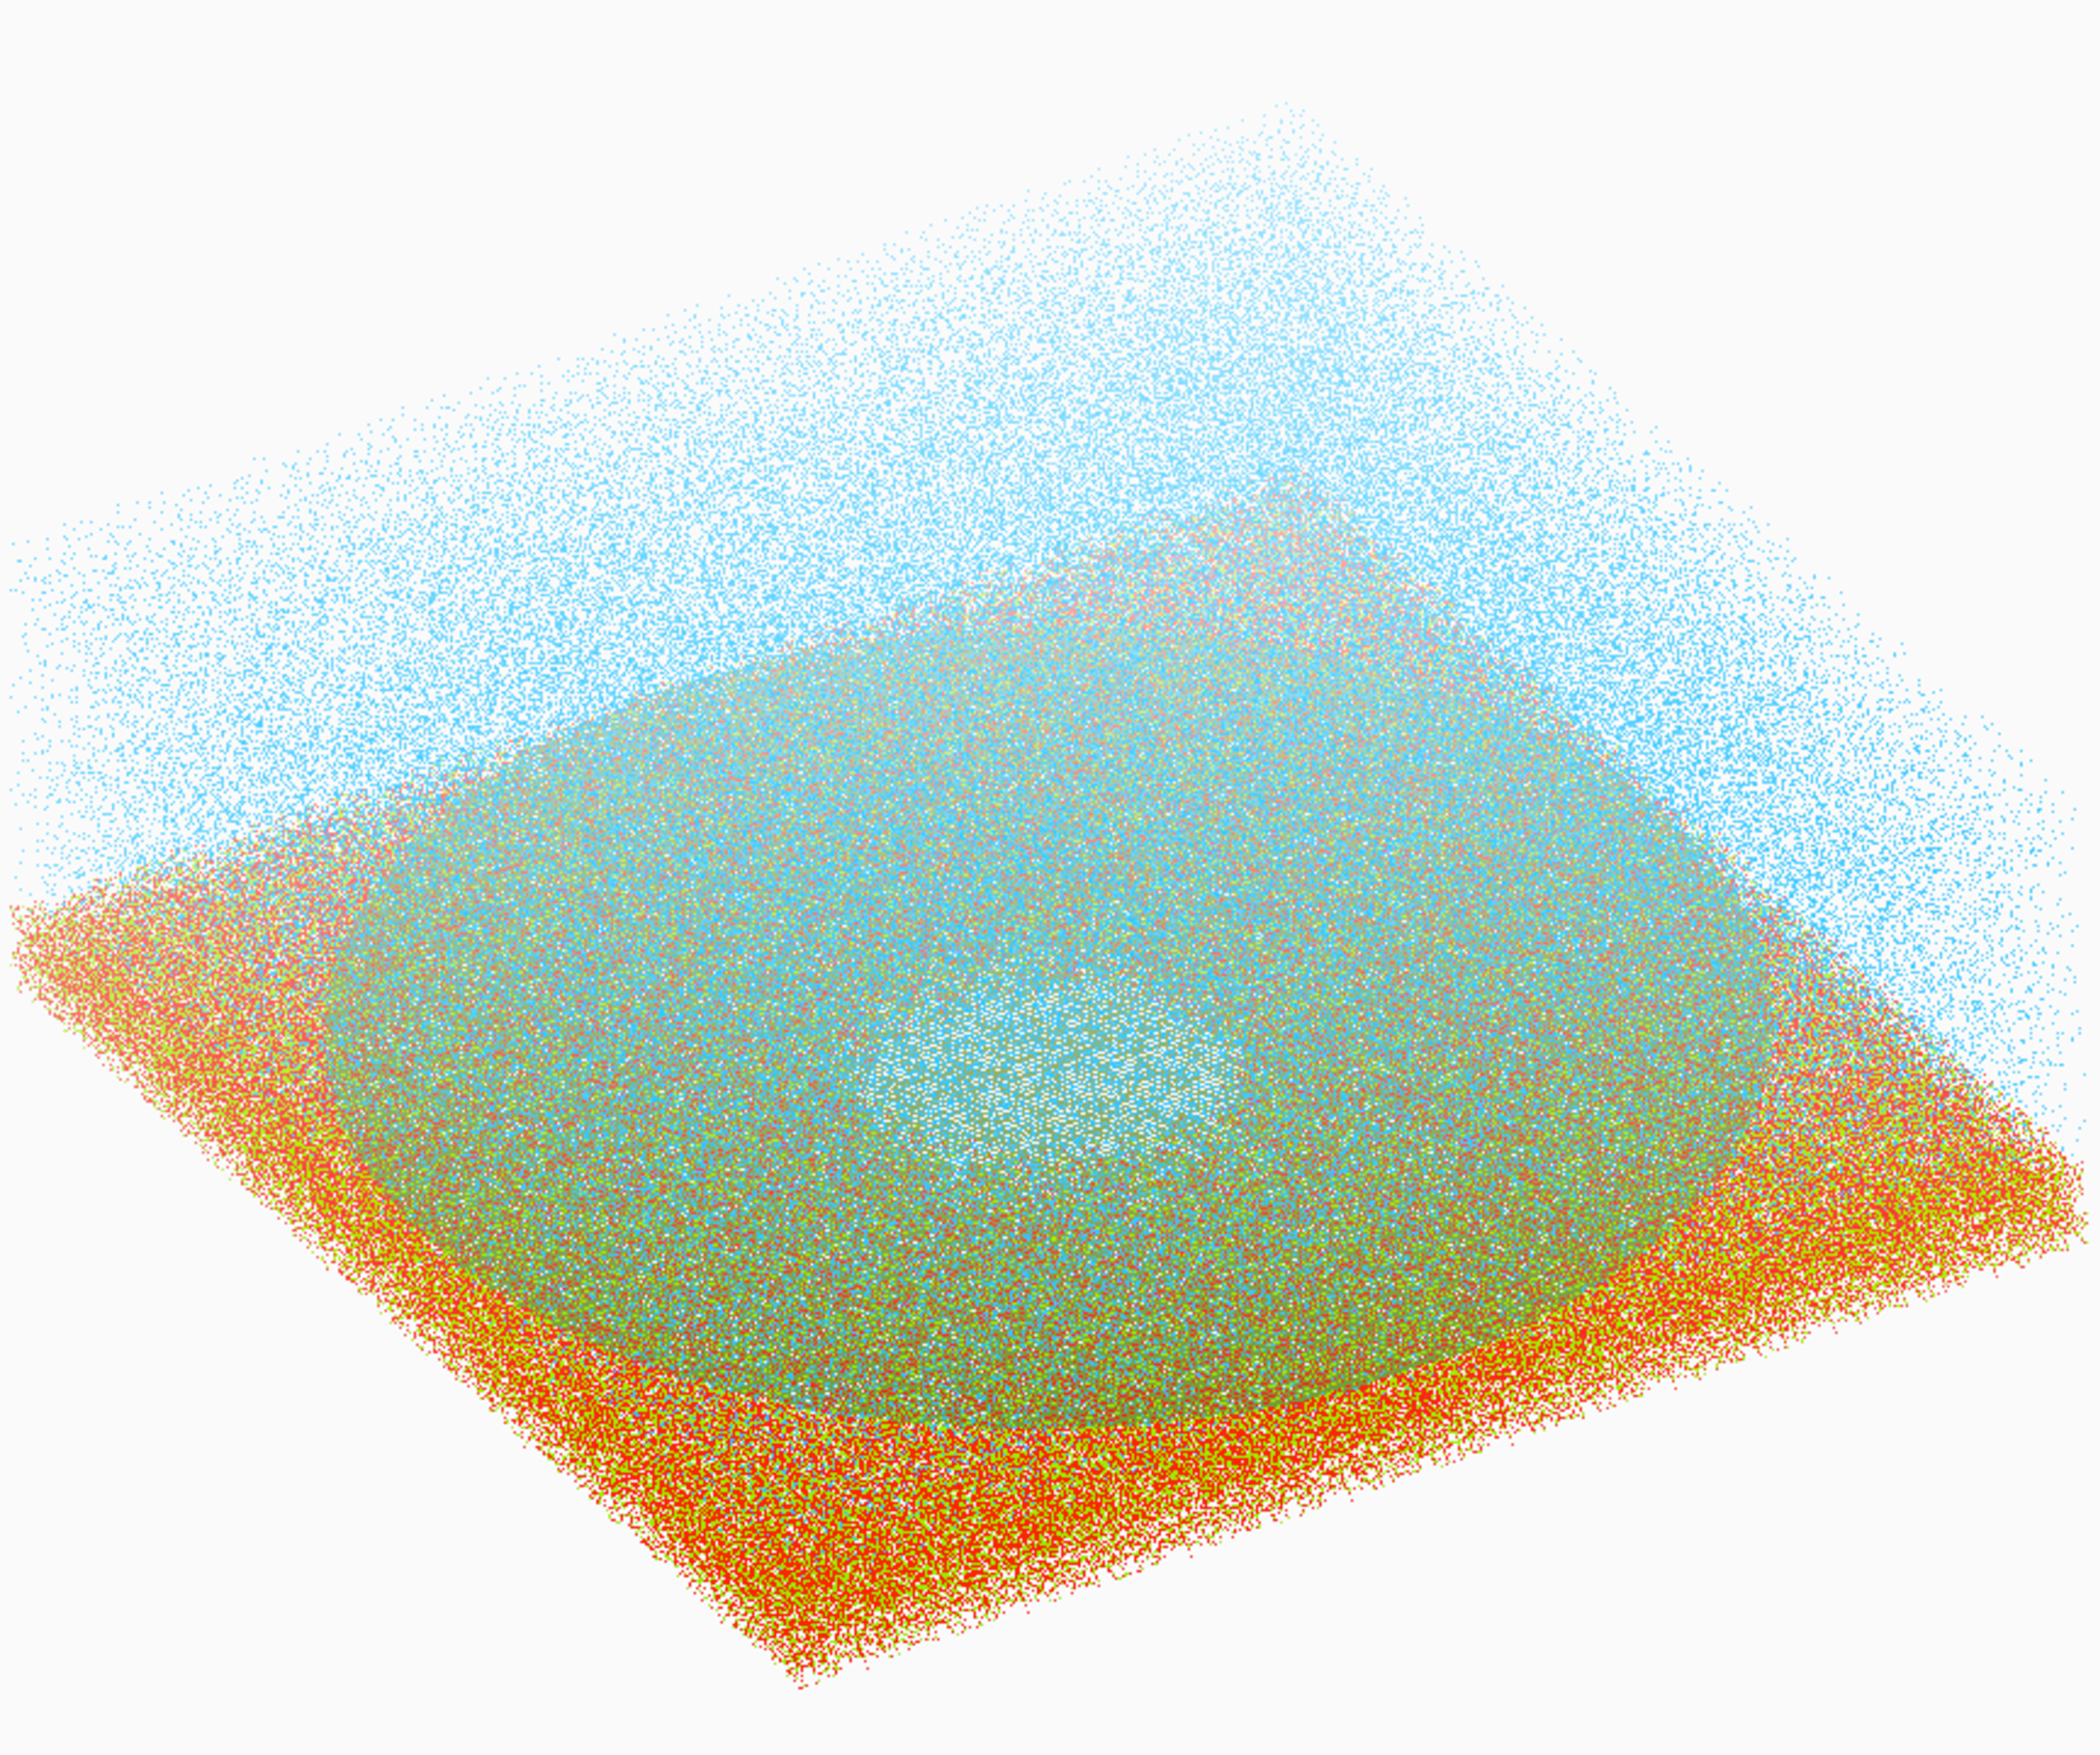
\includegraphics[scale=0.12]{Figs_Friction/MD.pdf}
	\end{center}
	\caption[Schematic diagram of the atomistic simulation]{\label{fig:fri:MD} Schematic diagram of the atomistic simulation of the pressurized graphene sealed microchamber including (from bottom to top) amorphous SiO$_{2}$ substrate (red and orange atoms), circular graphene monolayer (brown atoms) and argon gas (cyan atoms). Visualization was performed using Visual Molecular Dynamics \cite{Humphrey1996}.}
\end{figure}

The system was first relaxed at room temperature (300K) with a pressure of .03 MPa, at which point the gas density was slowly increased by reducing the volume of gas to increase the pressure.
When the desired deflection of graphene was reached, the gas density was then kept fixed, and the system was allowed to relax at that pressure for 10 ps.
The final equilibrium configuration of graphene was computed by averaging over all of the atomic positions of graphene during the relaxation period with constant gas density.
The substrate was assumed to be rigid and fixed during the simulation.
As a boundary condition on the graphene, the atoms in the outer 1 nm annulus of the supported graphene were fixed during the simulation matching the experimental observation that the supported graphene only slides in a local region around the hole, remaining fixed at large radii.
A canonical ensemble (NVT) at room temperature (300K) was used for the entire simulation and reflection boundary conditions were used to ensure that gas atoms remained inside the simulation box.  

To calculate the strain in the deformed graphene sheet, the atomistic displacement field was first found \cite{ZimmermanIJSS2009} by calculating the difference between the reference (initial) configuration and the final, deformed configuration.
The strain tensor from continuum mechanics was then calculated as
\begin{equation} \label{eq:fri:straindisp}
	\epsilon_{ij}=\frac{1}{2}\left(\frac{\partial {u_i}}{\partial {X_j}} + \frac{\partial {u_j}}{\partial {X_i}} + \frac{\partial{u_k}\partial{u_k}}{\partial{X_i}\partial{X_j}}\right),
\end{equation}
where $\epsilon_{ij}$ are the components of the strain, $u$ is the displacement, and $X$ denotes the position of a point in the reference configuration.

The displacement field $\mathbf{U}$ for each atom was computed by linearly interpolating, using standard finite element method shape functions for triangular elements \cite{hughes1987}.
The displacements of its three nearest neighbors is calculated as $\mathbf{U}=\mathbf{N}\bullet\mathbf{u_N}$, where $\mathbf{N}$ are the finite element shape functions and $\mathbf{u}_{N}$ are the displacements for each atom.
From the displacement field $\mathbf{U}$, the strain was calculated by taking derivative of $\mathbf{U}$ as $\mathbf{\epsilon}=\mathbf{B}\bullet\mathbf{u_N}$, where $\mathbf{B}=\frac{\partial \mathbf{N}}{\partial \mathbf{X}}$.
The atomistic data plotted in the paper was obtained from the MD simulation results by the method above, and was expressed in polar coordinates. 

\section{Fitting Raman spectra to the continuum model}
In conjunction with the measured Raman spectra, the extended continuum model can be used to determine the sliding friction, the Gr\"{u}neisen parameter, and the shear deformation potential.
A simple comparison of the strains predicted by the extended Hencky model to strains found by directly inverting the positions of the $G^+$ and $G^-$ peaks is not possible because of the finite size of the focused laser beam.
Instead, spectra are predicted by integrating against the system point spread function.
A set of spectra predicted for each point in the line scan can then be compared to the measured line scan spectra.
The best fit is found by predicting spectra for a series of different fitting parameters and choosing the one that best matches the measured spectra.
This is done quantitatively by choosing the spectra with the smallest $\chi^2$.
A detailed description of the fitting algorithm used as well as the determination of fitting error is presented in Appendix \ref{chap:Fit}.

Unlike the sliding friction, the Gr\"{u}neisen parameter and shear deformation potential should be the same for every line scan.
As such, they were included as fitting parameters in only the two lines scans which best defined $\beta$ based on the splitting of the supported graphene's G band just outside the edge of the microchamber: the $\sim 5 \mu m$ radius monolayer and the $\sim 5 \mu m$ radius trilayer at 0.80 MPa of applied pressure.
Figure \ref{fig:fri:gammabeta} shows reduced dimensionality plots of the $\chi^2$ per degree of freedom space.
As described in Appendix \ref{chap:Fit}, each data point in this type of plot represents the best case for the given value of the plotted fitting parameters.
The other, not plotted, fitting parameters ($\beta$ and $F$ for the $\gamma$ plot, and $\gamma$ and $F$ for the $\beta$ plot) are chosen to minimize $\chi^2$ at each data point.
The sharp minimum and the agreement between monolayer and trilayer indicates a good determination of $\gamma$ and $\beta$.
Using an increase in $\chi^2$ per degree of freedom of 0.25 to define uncertainties gives $\gamma_{mono} = 1.89 \pm .02$, $\gamma_{tri} = 1.89 \pm .02$, $\beta_{mono} = 0.69 \pm .04$, and $\beta_{tri} = 0.71 \pm .06$.
The averages of the monolayer and the trilayer, $\gamma=1.89 \pm 0.01$ and $\beta= 0.70 \pm 0.04$, were treated as known material parameters when fitting the remaining twenty Raman line scans.

\begin{figure}
	\begin{center}
	\newcommand{\sscale}{.8}
\begin{tikzpicture}[scale=\sscale]	
	\begin{scope}[xshift=-4.5 cm,yshift=0 cm]
		\node at (0,0) {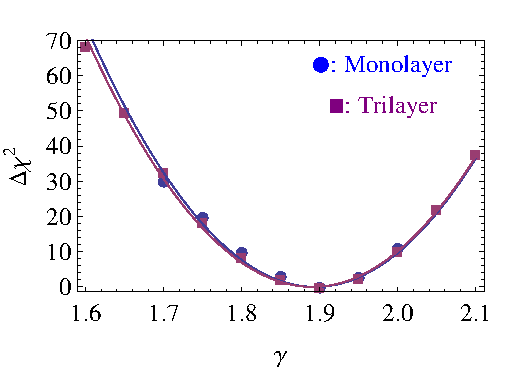
\includegraphics[scale=\sscale]{Figs_Friction/2012-12-11_Gbest.pdf}};
		\node at (-3.8,3) {\textbf{(a)}};
	\end{scope}
	
	\begin{scope}[xshift=4.5 cm,yshift=0 cm]
		\node at (0,0) {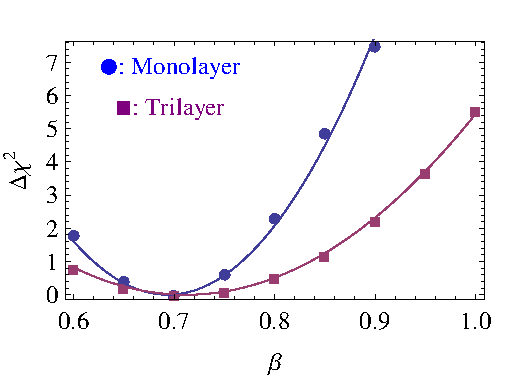
\includegraphics[scale=\sscale]{Figs_Friction/2012-12-11_Bbest.pdf}};
		\node at (-3.8,3) {\textbf{(b)}};
	\end{scope}
\end{tikzpicture}
	\end{center}
	\caption[Determination of the Gr\"{u}neisen parameter and shear deformation potential]{\label{fig:fri:gammabeta}Determination of the Gr\"{u}neisen parameter and shear deformation potential based on global fits to a monolayer covered (blue, circles) and a trilayer covered (purple, squares) $\sim 5 \ \mu m$ radius sealed microchamber at 0.80 MPa of applied absolute pressure.
	All three fitting parameters ($F$, $\gamma$, and $\beta$) were included in the fits.
	In (a) and (b) the reduced dimensionality plots of the deviation of $\chi^2$ per degree of freedom from the minimum are plotted for the Gr\"{u}neisen parameter and shear deformation potential respectively.
	The parabolic fits show sharp minimum.
	}
\end{figure}

Table \ref{tab:fri:gb} compares the measurements of the Gr\"{u}neisen parameter and shear deformation potentials to previous measurements.
The substrate on which the parameters were measured in also included.
Our measured $\gamma$ is commensurate with most of the other measured values and agrees particularly well with the \textit{ab initio} calculations of Cheng \textit{et al.} \cite{Cheng2011}.
On the other hand, the measured shear deformation potential is lower than most other measurements.
Buckling out-of-plane cannot explain this result since the mono and trilayers would buckle differently for a microchamber with the same pressure and radius.
These are the first measurements of $\gamma$ and $\beta$ for which the sliding of FLG over its substrate was included.

\begin{table}
	\begin{center}
	\begin{tabular}{l c  c }
		\hline
		\hline
		 & $\gamma$ & $\beta$ \\
		 \hline
		 This work & 1.89 & .70 \\
		 $\mathrm{SiO_2}$ depression \cite{Metzger2010} & 2.4 & \\
		 On PDMS \cite{Huang2009} & .69 & .38 \\
		 On SU8 \cite{Mohiuddin2009} & 1.99 & .99\\
		 Embedded \cite{Frank2010} & 2.01 & 1.01 \\
		 On Acrylic \cite{Yoon2011} & 2.2 & .93\\
		 Bubble \cite{Zabel2012} & 1.8 \\
		\textit{Ab initio} \cite{Thomsen2002} & 2.0 & 0.66 \\
		\textit{Ab initio} \cite{Cheng2011} & 1.86 & .96\\
		 \hline
		 \hline
	\end{tabular}
	\end{center}
	\caption[Summary of the Gr\"{u}neisen parameter, $\gamma$, and shear deformation potential, $\beta$, as measured on different substrates]{\label{tab:fri:gb} Summary of the Gr\"{u}neisen parameter, $\gamma$, and shear deformation potential, $\beta$, as measured on different substrates.}
\end{table}

The extended Hencky model agrees extremely well with the measured spectra.
Figure \ref{fig:fri:fitlinescan} shows a global data fit for a $\sim 5 \ \mu m$ radius monolayer covered graphene sealed microchamber at 0.80 MPa of applied pressure.
The spectra and fits from each position along the line scan are stacked vertically in the direction of the line scan.
The extended continuum model successfully fits the softening and splitting of the G band of the supported graphene and successfully predicts the downshift and sharpening of the G band of the suspended graphene as the center of the microchaber is approached.
In comparison, without the theoretical extension the standard Hencky model would fail to reproduce the supported graphene spectra.

\begin{figure}
	\begin{center}
	\begin{tikzpicture}[scale=.75]
	%The spectra
	\node at (0,0) {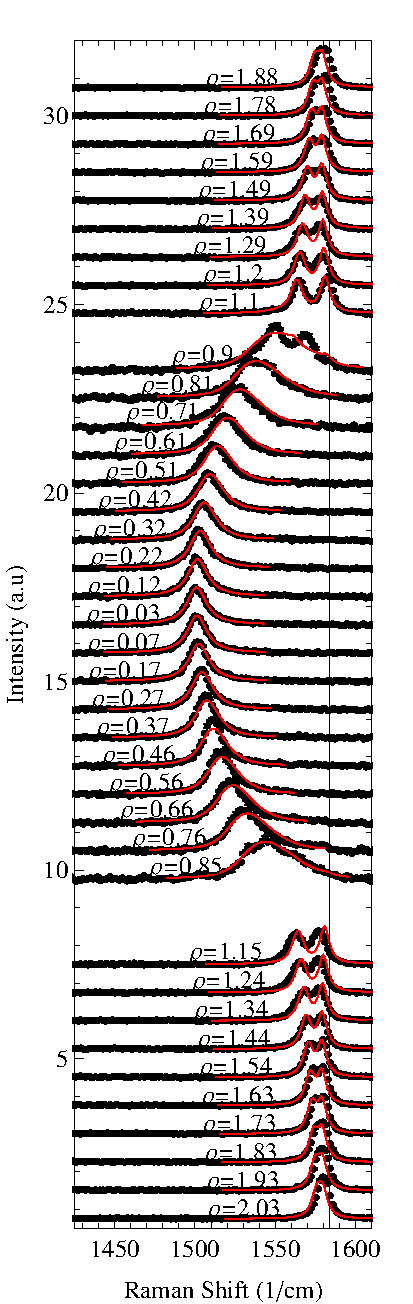
\includegraphics[scale=.75]{Figs_Friction/2012-12-18_Fit_101psi_Spectra_for_paper.pdf}};
	
	%The picture of the hole
	\newcommand{\arrowlength}{.44*1.2*1.77 cm}
	\begin{scope}[xshift=1.7 cm,yshift=.7 cm]
		%For the total scale=1 the .jpg scale is .6
		\node at (0,0) {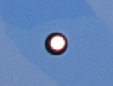
\includegraphics[scale=.8,angle=-90,trim=9.5mm 8.5mm 9.5mm 8.75mm,clip]{Figs_Friction/SB02_1_cropped.jpg}};
		\draw[->,black,thick,>=stealth] (0,-\arrowlength) -- (0,\arrowlength);
	\end{scope}
\end{tikzpicture}]
	\end{center}
	\caption[Raman spectra from a line scan over a $\sim 5 \ \mu m$ radius monolayer graphene sealed microchamber with 0.80 MPa of applied pressure analyzed with the extended Hencky model (red lines)]{\label{fig:fri:fitlinescan} Raman spectra from a line scan over a $\sim 5 \ \mu m$ radius monolayer graphene sealed microchamber with 0.80 MPa of applied pressure analyzed with the extended Hencky model (red lines).  The spectra taken along the path shown in the inset are arrayed vertically with spectra taken too close to the edge of the microchamber omitted (see text).  The black vertical line is positioned at the supported graphene's unstrained G band energy.}
\end{figure}

\section{Measured frictional dependencies}
The sliding friction extracted for eight microchambers with radii between 1.2 and 5 $\mu m$ and with applied absolute pressures from 0.10 to 0.80 MPa exhibits fundamentally different behavior for trilayer graphene than for monolayer and bilayer.
In Figure \ref{fig:fri:FvsP}a (left) the friction is plotted as a function of absolute applied pressure.
The data for trilayer graphene (black dots) shows a linearly dependent sliding friction in accordance with Amontons' law with a coefficient of friction of $0.11 \pm 0.01$.
For reference, Teflon on Teflon has $\mu=0.04$ while clean steel on clean steel has $\mu=0.6$ \cite{Resnick2002}.
A zoom in of the trilayer data is shown in Figure \ref{fig:fri:trimu}.
The sliding friction for monolayer and bilayer graphene behave much differently.
They decrease generally with applied pressure and the wide scatter of the points for different radii and layer number clearly indicate that the sliding friction is dependent on the geometry of the microchamber.
Our theoretical analysis shows that the radial strain at the edge due to the pressure pushing the graphene into the microchamber has the same radii and layer number dependence as the friction, so the sliding friction is replotted as a function of the radial strain in Figure \ref{fig:fri:FvsP}b (right).
The monolayer and bilayer data for all different radii microchambers now \emph{collapse} to a single curve versus radial strain, well described by $1/\epsilon_{r,edge}$ behavior (dashed line).
The best fit to the strain dependence is $0.002 MPa/\epsilon_{r,edge}$.

\begin{figure}
	\begin{center}
	\begin{tikzpicture}[scale=.9]
	%The spectra
	\node at (0,0) {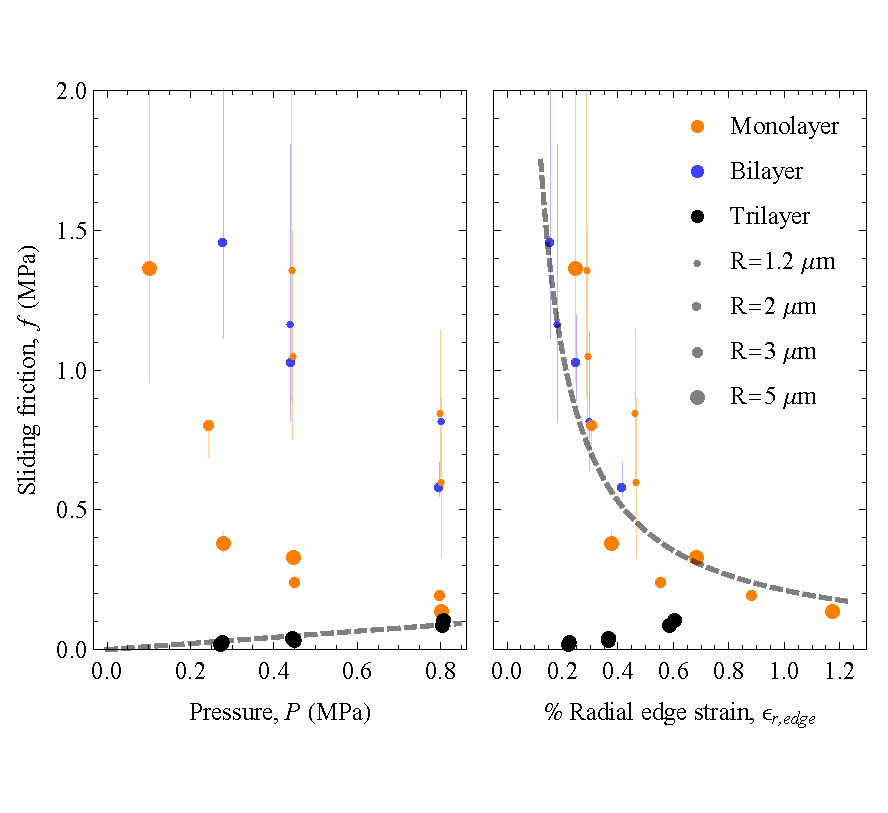
\includegraphics[scale=.9]{Figs_Friction/FvsP.pdf}};
	\node at (-5.8,5.75) {\textbf{a}};
	\node at (.95,5.75) {\textbf{b}};
\end{tikzpicture}
	\end{center}
	\caption[The dependencies of sliding friction for FLG]{\label{fig:fri:FvsP}
	The dependencies of sliding friction for FLG extracted by analyzing Raman line scans with the extended Hencky model.
	In panel (a) (left) friction is plotted as a function of absolute applied pressure where in panel (b) (left) it is plotted as a function of the radial strain at the edge of the microchamber.
	The size of each data point represents the radius of the FLG-sealed microchamber corresponding to that point. The error bars are given by an increase in global fit $\chi^2$ per degree of freedom of 0.25.
	The sliding friction of trilayer graphene depends linearly on the absolute applied pressure in agreement with Amontons' law.
	The sliding friction of monolayer and bilayer graphene, however, go as the inverse of the radial strain at the edge of the microchamber.
	Gray dashed lines are the best fits to these trends.}
\end{figure}

\begin{figure}
	\begin{center}
	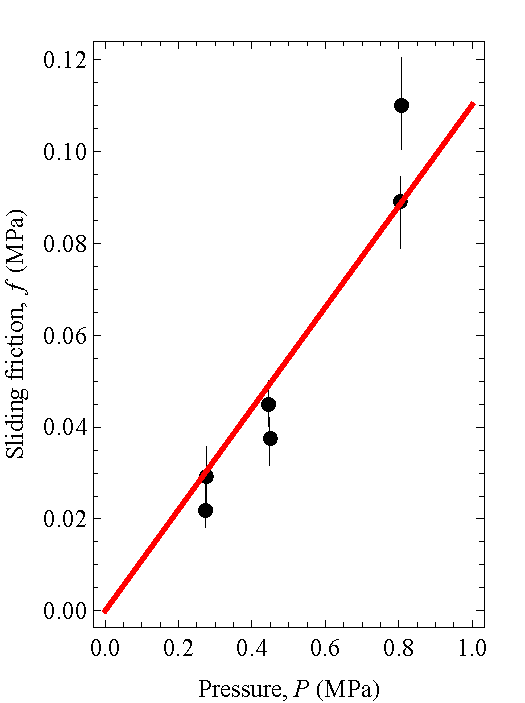
\includegraphics{Figs_Friction/Tri_mu.pdf}
	\end{center}
	\caption[The sliding friction for trilayer graphene as a function of the absolute applied pressure]{\label{fig:fri:trimu} The sliding friction for trilayer graphene as a function of the absolute applied pressure extracted from Raman lines scans over two $5 \ \mu m$ radii trilayer sealed microchambers.
	The datat is fit with Amonton's law, $f=\mu P_{abs}$, giving a coefficient of friction between trilayer graphene and $\mathrm{SiO_2}$ of $\mu=0.11 \pm 0.01$. }
\end{figure}

The gross difference in behavior between trilayer on one hand, and mono-and bilayer on the other, illustrates the two roles of the applied pressure.
The pressure load pushes the graphene more firmly onto the substrate so that sliding friction should increase (Amontons' law), yielding a positive coefficient of friction.
This is the case for the trilayer graphene.
On the other hand, as the pressure pushes the graphene into the microchamber, it creates a radial tension in the supported graphene outside the microchamber.
The data collapse in Figure \ref{fig:fri:FvsP}b for monolayer and bilayer graphene demonstrate that the pressure dependence of the sliding friction is not due to loading the supported graphene but is instead due to the graphene being pulled and stretched by the applied pressure.
This is the only mechanism that would depend on the geometric parameters of the microchamber while also being consistent with the data.
It is not surprising that the sliding friction for mono- and bilayer graphene is dependent on the strain and not the load because thin graphene conforms nearly perfectly to a $\mathrm{SiO_2}$ substrate \cite{Stolyarova2007,Lui2009,Cullen2010}.
Increasing the load cannot further increase the contact area, but increasing the radial strain beyond the edge of the microchamber may act to smooth out the graphene sheet, decreasing the contact between the graphene and the substrate, and thus decreasing the sliding friction.
The bending rigidity, which goes as thickness cubed, of trilayer graphene must be high enough to counteract the adhesion energy, causing lower conformation and allowing for a traditional pressure and load response.
The existence of a bilayer to trilayer crossover in FLG-substrate interactions is also observed in GPa range pressure measurements of silicon dioxide supported graphene \cite{Proctor2009,Nicolle2011}.
Nicolle \textit{et al.} observed a decrease in the pressure response of the G band between bilayer and trilayer graphene which was attributed to the transition from biaxial compression mediated by the substrate to hydrostatic compression mediated by the pressure transmitting medium \cite{Nicolle2011}.

\section{Summary}
In summary, it has been demonstrated that few layer graphene slides along the substrate when pulled.
Furthermore, using a newly developed extension of the continuum Hencky model, the sliding friction as a function of the number of atomic layers and the load was extracted.
Trilayer graphene shows a typical load response whereas the sliding friction for monolayer and bilayer graphene goes as the inverse of strain.
The data collapse of the friction for mono- and bilayer graphene when plotted versus strain is strong experimental evidence for a reduction in surface conformation when graphene is pulled as the fundamental origin of the negative coefficient of friction.
These results will be important for the design of strain engineered devices \cite{Pereira2009a}, while the sliding of a flexible surface along a bulk object should be of fundamental, tribological interest.
Finally, the method used in generalizing Hencky's solution should be useful for including distributed strains in other continuum models for use in designing strain-engineered graphene devices and in understanding other, few-layer material systems.